\chapter{Primer núcleo: Reconocimiento Automático de Patentes (ALPR)} \chapterlabel{Cap_Patentes} \label{cap:alpr}

\section{Introducción}\label{sec:introALPR}
En el desarrollo del prototipo, el reconocimiento de la patente, tanto del vehículo que ingresa  como del que egresa, es una de las etapas fundamentales.

El reconocimiento automático de patentes es un problema típico que involucra varias ramas de estudio, principalmente al área de Reconocimiento de Patrones y el campo de la Visión artificial, y que ya ha sido estudiado ampliamente \cite{TRA-147} \cite{0a392c343021f65fa374375e148cb5770a88} \cite{2011-Reconocimiento_automatico_de_numero_de_patente} \cite{13EM9}.

Una de las principales dificultades que se presentan es que los escenarios pueden ser cambiantes, como podía ocurrir en el caso de un Sistema de Transporte Inteligente (ITS), donde el reconocimiento de patentes permite identificar vehículos en movimiento y obtener varias matriculas simultáneamente. \cite{0a392c343021f65fa374375e148cb5770a88} \cite{LicensePlates2018}.

En nuestro caso, a pesar de que se considera que el sistema puede aplicarse a diversos tipos de estacionamientos, el escenario es más acotado: la cámara se encuentra en una posición fija y el vehículo frenando a baja velocidad. En este contexto, se tienen en cuenta otras posibles problemáticas, como las variaciones lumínicas (día/noche), la iluminación propia de la placa y la existencia de distintos modelos de placas patentes en nuestro país: argentina antigua (1995 - 2016) y Mercosur (2016- presente). Además, se consideran diferentes tipos de vehículos: automóviles, camionetas y motocicletas.

El uso de un sistema que recoja los datos de la matrícula de un vehículo y lo almacene en una base de datos en formato de texto evita la necesidad de ocupar espacio de memoria debido al almacenamiento de videos o imágenes y facilita la consulta de los datos de cada uno de los clientes del establecimiento en el que se monte el mismo.

El objetivo de este capítulo es presentar todo lo relacionado con el desarrollo del sistema reconocedor de patentes para el Sistema Automatizado de Estacionamientos SAE. Se describen las características generales de los sistemas ALPR, los tipos de software disponibles, el sistema elegido, la parametrización e implementación del mismo, las características de los conjuntos de datos utilizados y las características principales del sistema implementado, como el tratamiento de video. 

\section{Sistemas de Reconocimiento Automático de Patentes ALPR}\label{sec:sysALPR}

\subsection{Estado del arte}
La detección de patentes de vehículos de manera automática, puede ser utilizada en varias aplicaciones como el multado de vehículos, el control de accesos y sistemas de seguridad, entre otras. Es por eso que en la actualidad existe una amplia cantidad de empresas dedicadas al reconocimiento de patentes. Entre ellas, podemos destacar a PIPS TECHNOLOGY, empresa fundada en el Reino Unido que ofrece no solo las aplicaciones previamente mencionadas, sino que además posee un sistema de transporte inteligente, control de congestionamiento, entre otras \cite{pipstechnology} . Por otra parte, se encuentra la empresa canadiense GENETEC, la cual, al igual que la anterior, ofrece soluciones de ALPR ya mencionadas como los sistemas de seguridad y el control de accesos \cite{genetec}. Por último, Neural Labs es una empresa radicada en Barcelona, España. Además de las aplicaciones ya mencionadas, la misma utiliza el reconocimiento de patentes para el control de clientes en gasolineras y peajes \cite{neurallabs}.

Particularmente en Argentina, si bien los sistemas ALPR son utilizados en algunas aplicaciones como el control de flujo o el multado, los mismos no se encuentran ampliamente difundidos, como es el caso en el plano internacional. Dentro de nuestro país, podemos mencionar la compañía VISART, la cual es una de las pocas empresas nacionales que se encuentra trabajando en el área \cite{visart}.
Además, en Argentina, aun no se han logrado grandes avances acerca del uso de sistemas ALPR en playas de estacionamiento. Por lo tanto, la implementación desarrollada en este proyecto final resulta innovadora para nuestro país.

%ALPR son las siglas en inglés del reconocimiento automático de patentes (Automatic license plate recognition). Otra manera de llamarlo es ANPR, cuyo significado es Automatic number plate recognition. El mismo consiste en la extracción de información de la patente de un vehículo a partir de una imagen. 

%Fue inventado en el año 1976 por la División de Mejora Científica de la Policía británica, pero no se popularizó hasta la década de los 90, cuando el software se hizo más sencillo de manejar y el hardware más accesible \cite{anprInt}. Actualmente, está siendo muy utilizado para diversos propósitos tales como sistemas de seguridad, estacionamientos, controles de accesos en barrios cerrados y edificios, etc. 

%Hoy en día hay una gran cantidad de herramientas disponibles que permiten realizar el reconocimiento. Las mismas pueden ser tanto “open source” (software libre) como de origen comercial. Todas estas herramientas tienen un principio de funcionamiento similar y deben ser adaptadas al lugar en el que se las pretende utilizar. Esto se debe a que las patentes de los diferentes países, estados o provincias pueden tener diferentes fuentes, colores o estar escritas en distintos idiomas. 

%Actualmente existen numerosos trabajos realizados acerca del ALPR, en los cuales cada autor lo aborda desde su perspectiva y aporta sus descubrimientos, problemáticas y resultados al investigar y experimentar  con él \hl{[ac\'a podr\'ia repetir algunas de las referencias del 2do p\'arrafo de la intro]}. 

\subsection{Etapas generales de los sistemas ALPR} \label{key:etapasgenerales}
El proceso realizado por todo sistema ALPR involucra una serie de etapas generales que pueden ser llevadas a cabo a partir de diferentes metodologías \cite{TRA-147} \cite{LicensePlates2018} \cite{UCC4791_01}. Las mismas son las que se muestran en la figura~\ref{fig:Et_gen}, y se las describe a continuación:

\begin{figure}[H]
	\centering
	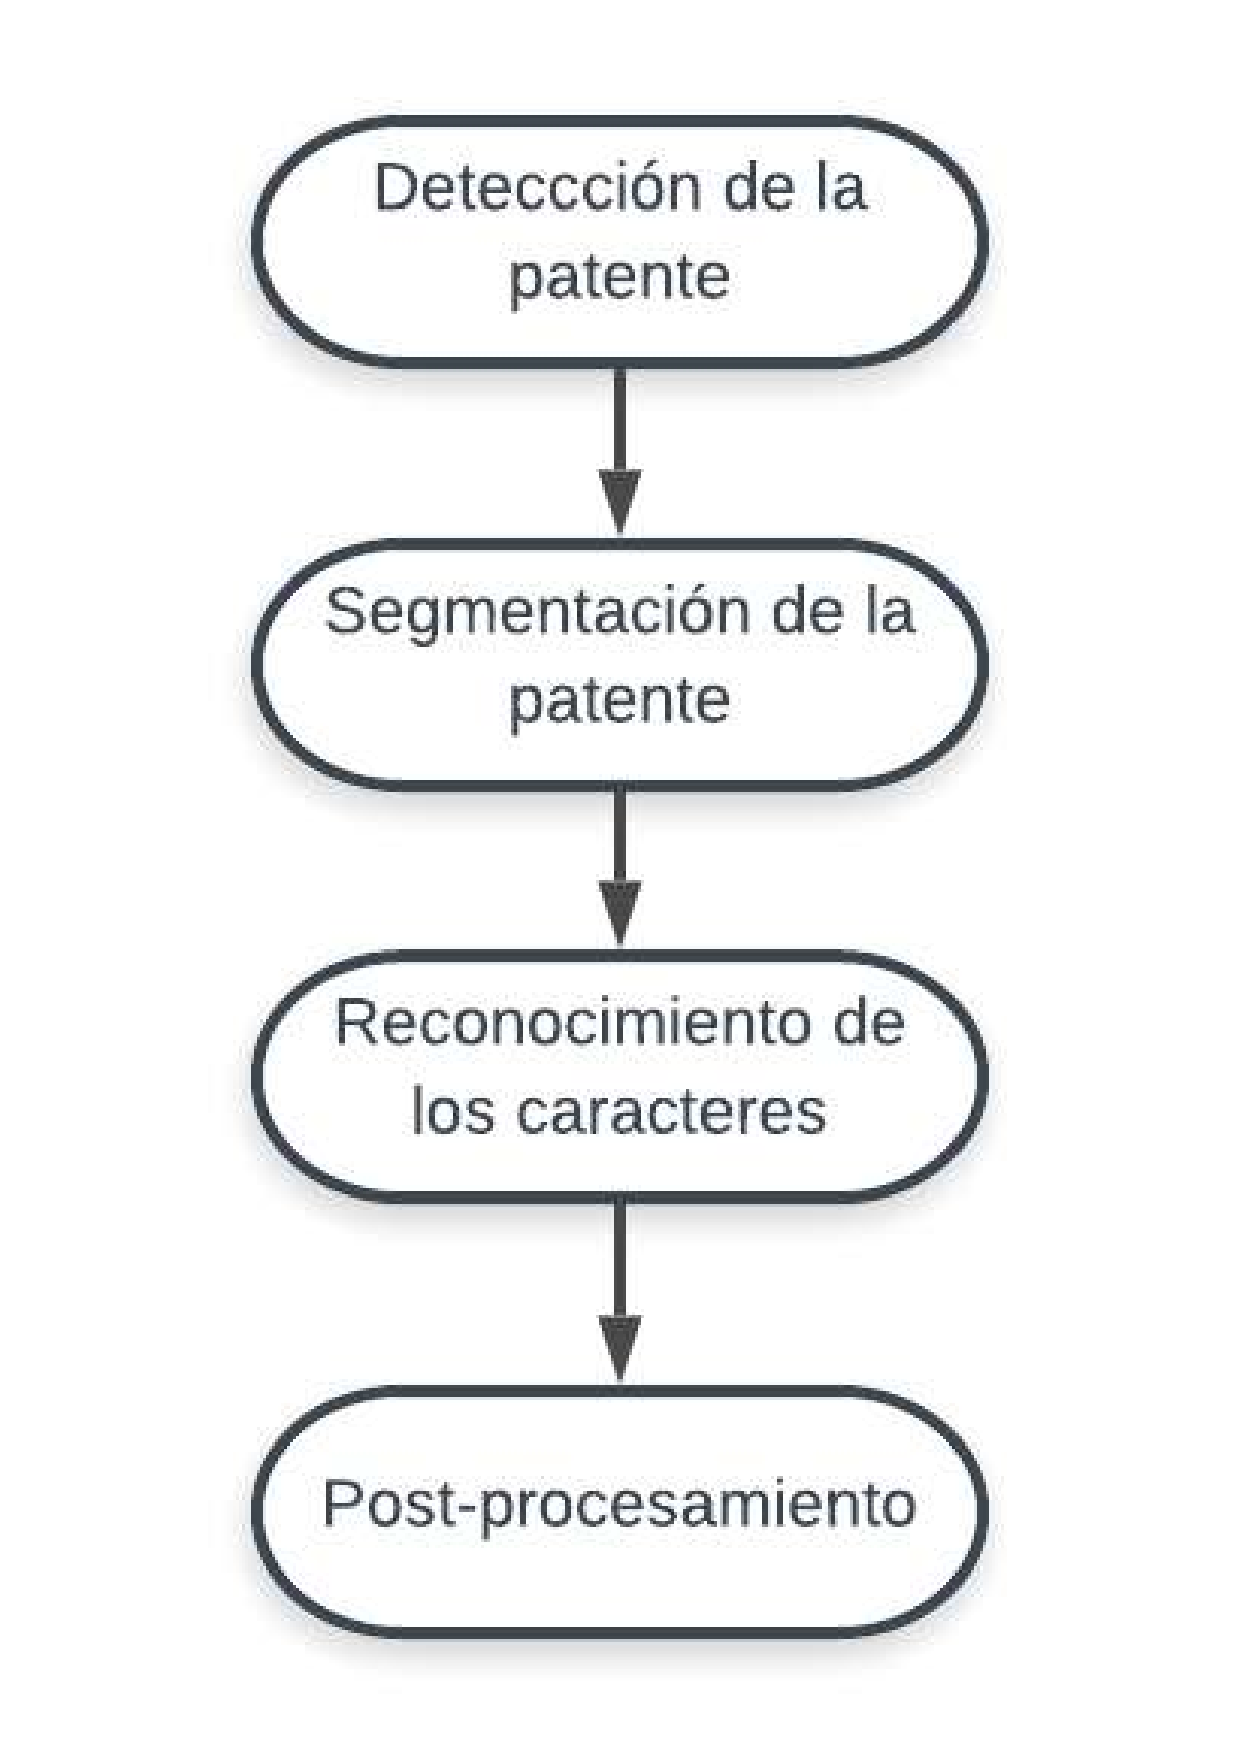
\includegraphics[scale=0.3]{Etapas_generales.pdf}
	\caption{Etapas generales de un sistema ALPR \cite{LicensePlates2018}.}
	\label{fig:Et_gen}
\end{figure} 

\noindent \textbf{Etapa 1: Detección de la patente}

Esta etapa depende en gran medida de ciertas características de la placa tales como forma, color, dimensiones, etc. Además, esta fase es afectada por las condiciones del entorno: iluminación, calidad de la cámara con la que se captura la imagen o video, las características del ambiente, etc. Normalmente, incluye una etapa de pre-procesamiento que prepara la imagen para el proceso de reconocimiento. 

El pre procesamiento consiste en la aplicación de diferentes procedimientos a la imagen, los cuales pueden variar dependiendo el algoritmo de detección que se utilice. Entre estos podemos destacar: 

\begin{itemize}
	\item \textbf{Transformación en una imagen en escala de grises:}
si la imagen a analizar se encuentra por ejemplo a color (RGB), contiene información que no es relevante, ya que el análisis de características para la identificación se realiza sobre una extracción de información acerca del valor numérico de intensidad de cada pixel y no de acuerdo al color que representa. Por lo tanto, los pixeles de la imagen transformada toman valores entre 0 y 255 pasando por las diferentes tonalidades de grises, donde 0 equivale al color negro y 255 al blanco.  Esto se observa en la figura~\ref{fig:img_grey}.

\item \textbf{Binarización:}
se realiza a través de métodos como el de Wolf Jolion \cite{wolf2004} y el de Otsu \cite{Image_Binarization_using_Otsu_Thresholdi}, entre otros. La binarización consiste en una reducción de información de una imagen digital en la que los únicos valores posibles son verdadero (1) o falso (0), los cuales corresponden a los colores blanco y negro respectivamente. Para determinar a cuál de estos valores corresponde la información de cada pixel, en el proceso de binarización se establece un umbral, que es un valor dentro de la escala de grises (0 a 255). El mismo es comparado con el valor de cada pixel y si este supera dicho umbral será un 1 y en caso contrario un 0. Además, cabe destacar, que también se pueden especificar umbrales en base a otra tonalidad, si es que se busca un objeto de un color especifico. Mediante esta técnica pueden separarse objetos o regiones que pueden ser de interés, del resto de la imagen. El resultado puede verse en la figura ~\ref{fig:img_bin}.


\item \textbf{Aplicación de filtros:}
pueden ser utilizados tanto para la remoción del ruido de la imagen como también, para realzar detalles de la misma antes de procesarla \cite{navacerrada}.
\end{itemize}

El paso siguiente es identificar la patente en la imagen, mediante algún algoritmo de detección como por ejemplo “edge detection”, “template matching” o “Artificial Neural Network” (ANN) \cite{LicensePlates2018}\cite{0a392c343021f65fa374375e148cb5770a88}. Estos algoritmos de detección, pueden combinarse con los métodos de multiescalamiento y/o ventana deslizante para encontrar la patente, independientemente del tamaño que esta posea, dentro de la imagen. 
Una vez identificada la patente en la imagen se la extrae para aplicarle una transformación a escala de grises y, luego, se la binariza con el objetivo de resaltar en blanco los caracteres y los bordes de la misma. Esto se observa en la figura~\ref{fig:img_prepro}.

\begin{figure}[H]
	\centering
	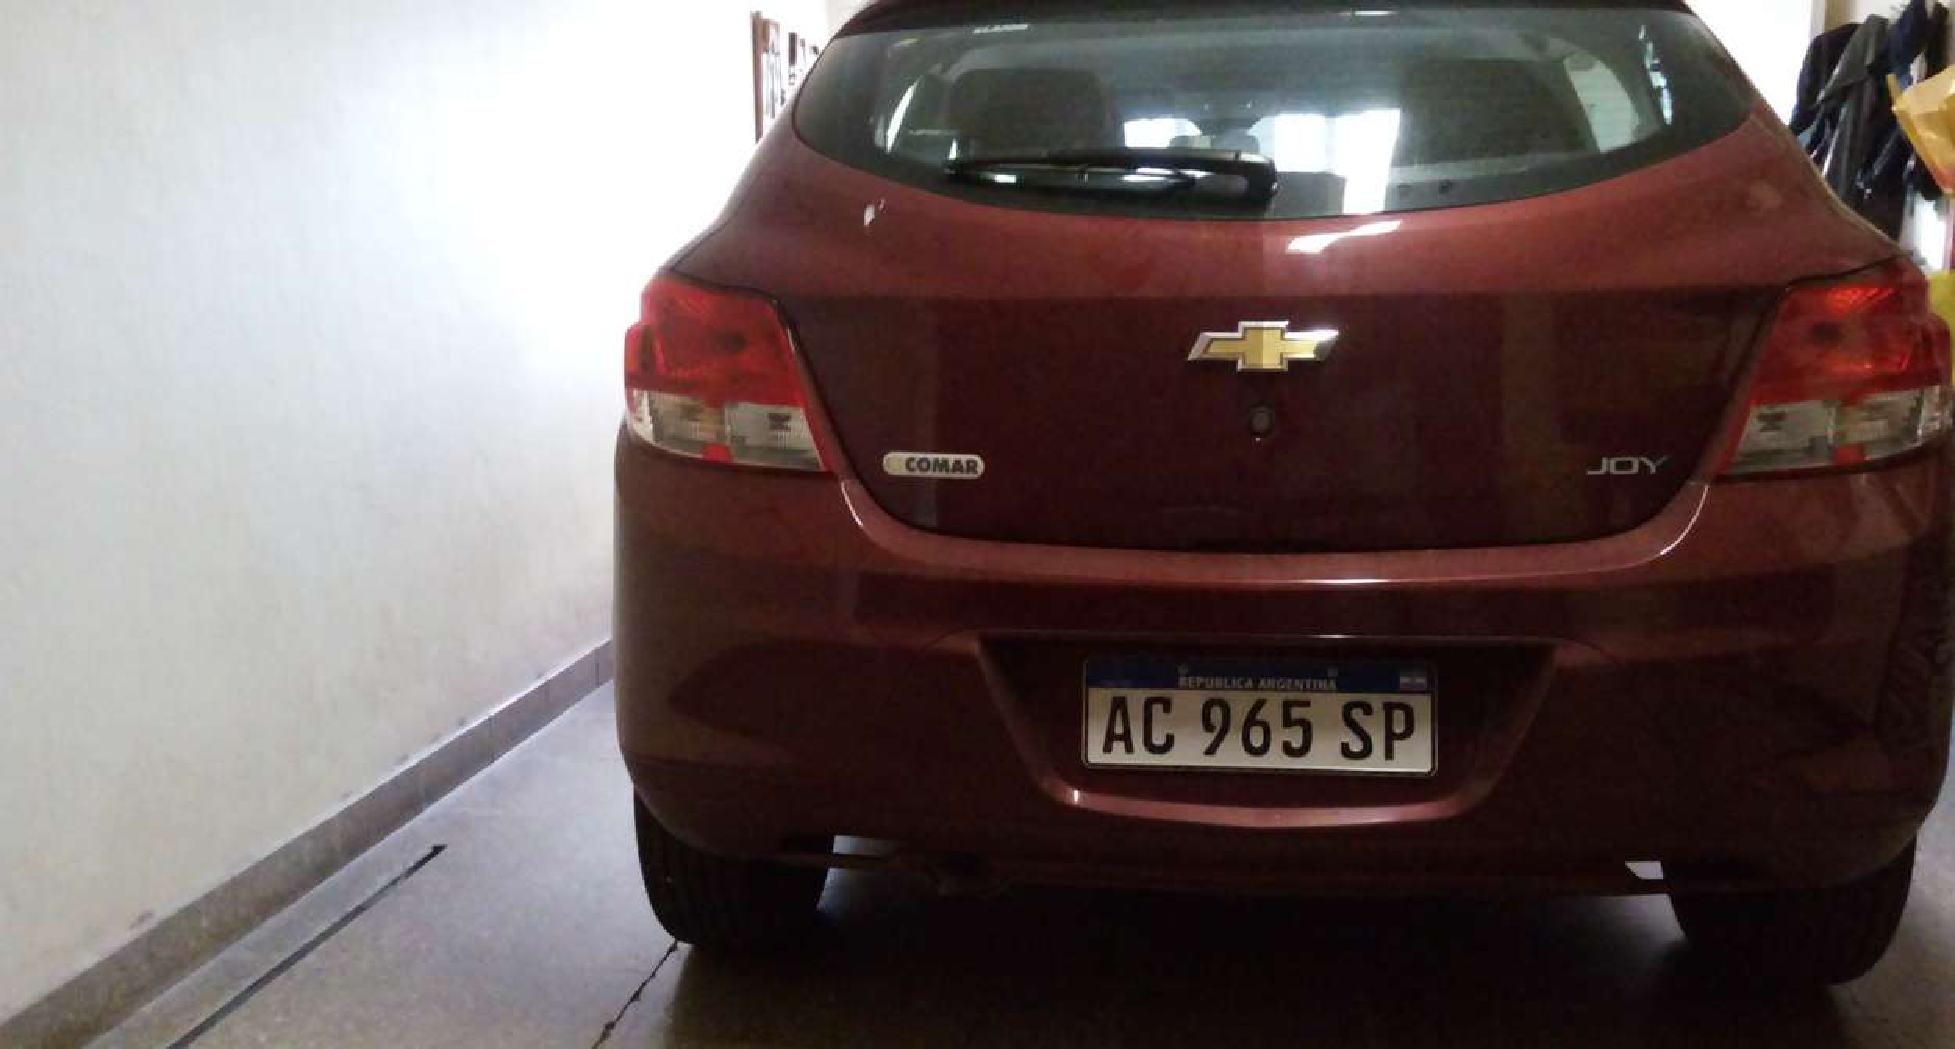
\includegraphics[scale=0.35]{imagen_original.pdf}
	\caption{Imagen del vehículo que posee la patente a analizar, antes de comenzar el proceso de reconocimiento.}
	\label{fig:img_orig}
\end{figure}
\begin{figure}[H]
	\centering
	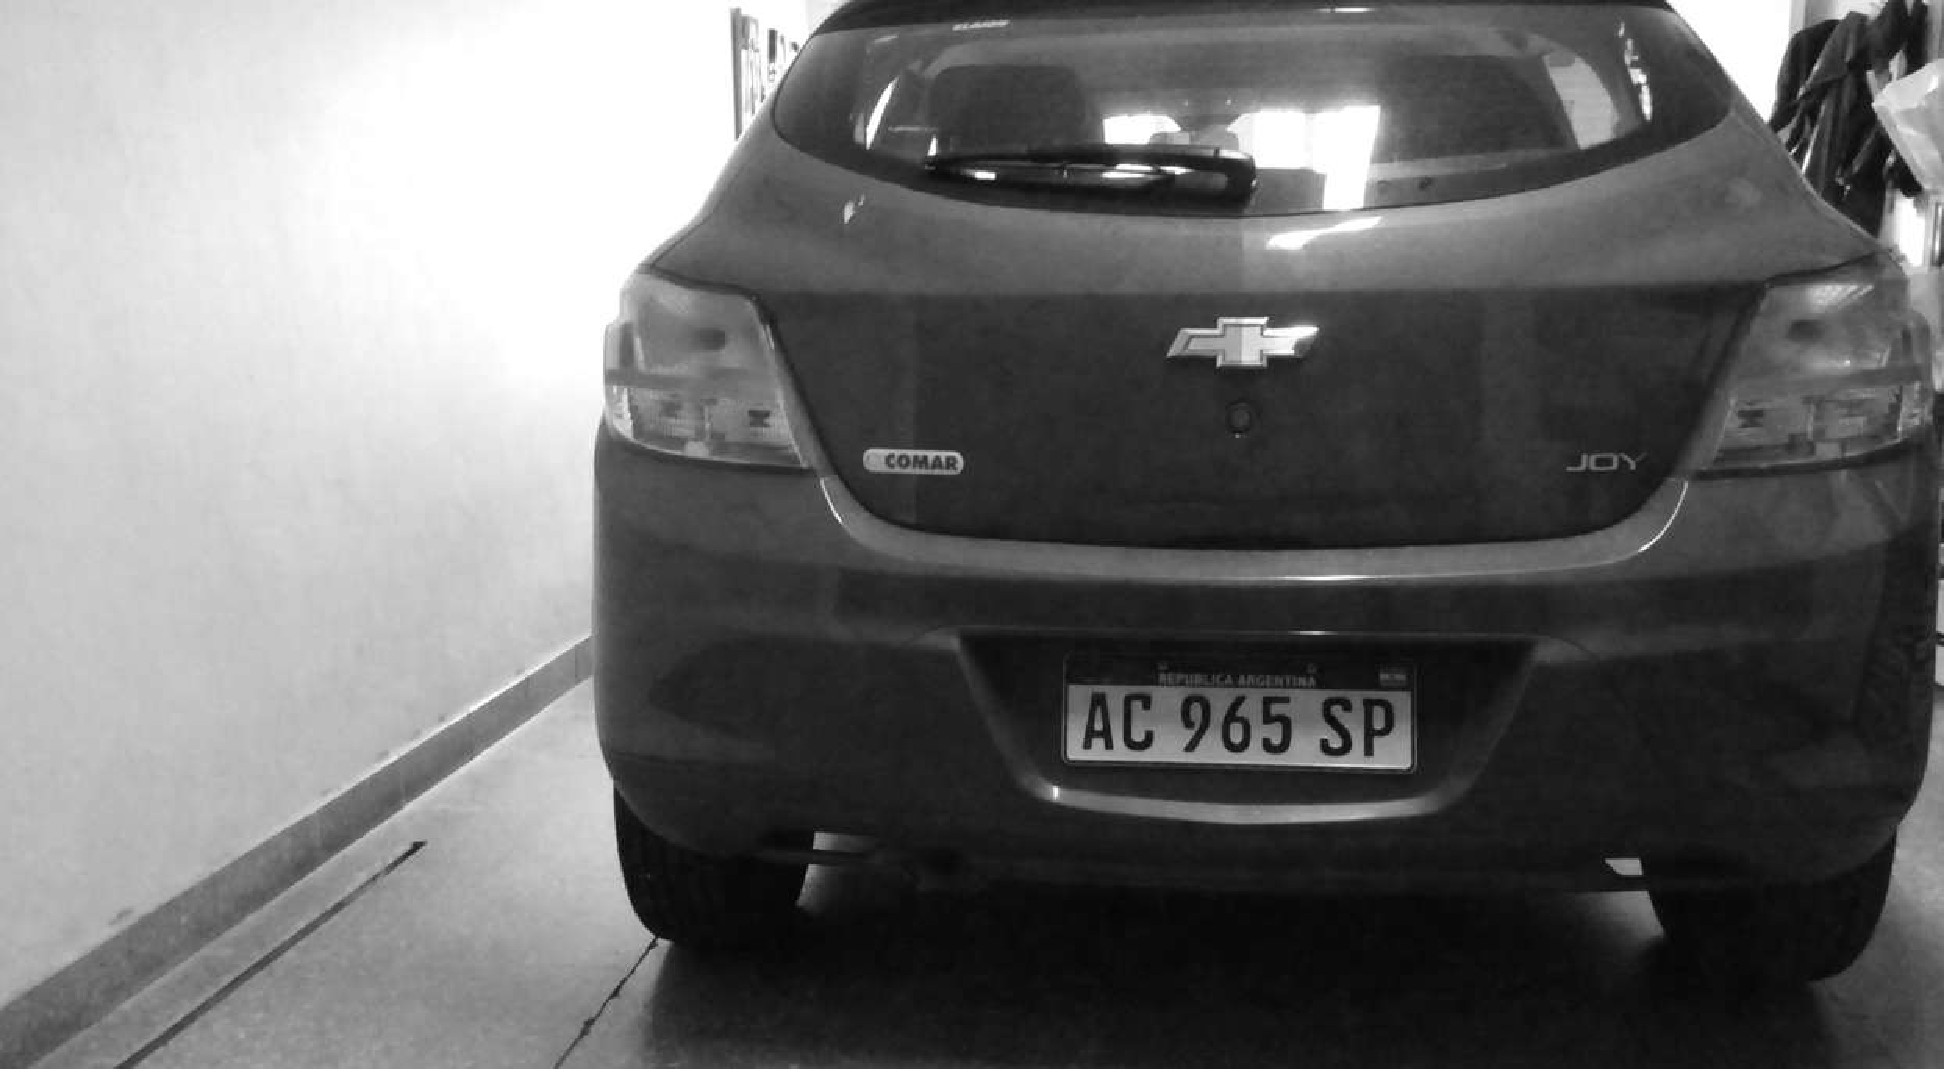
\includegraphics[scale=0.35]{escala_de_grises.pdf}
	\caption{Imagen del vehículo que posee la patente a analizar, en escala de grises.}
	\label{fig:img_grey}
\end{figure} 
\begin{figure}[H]
	\centering
	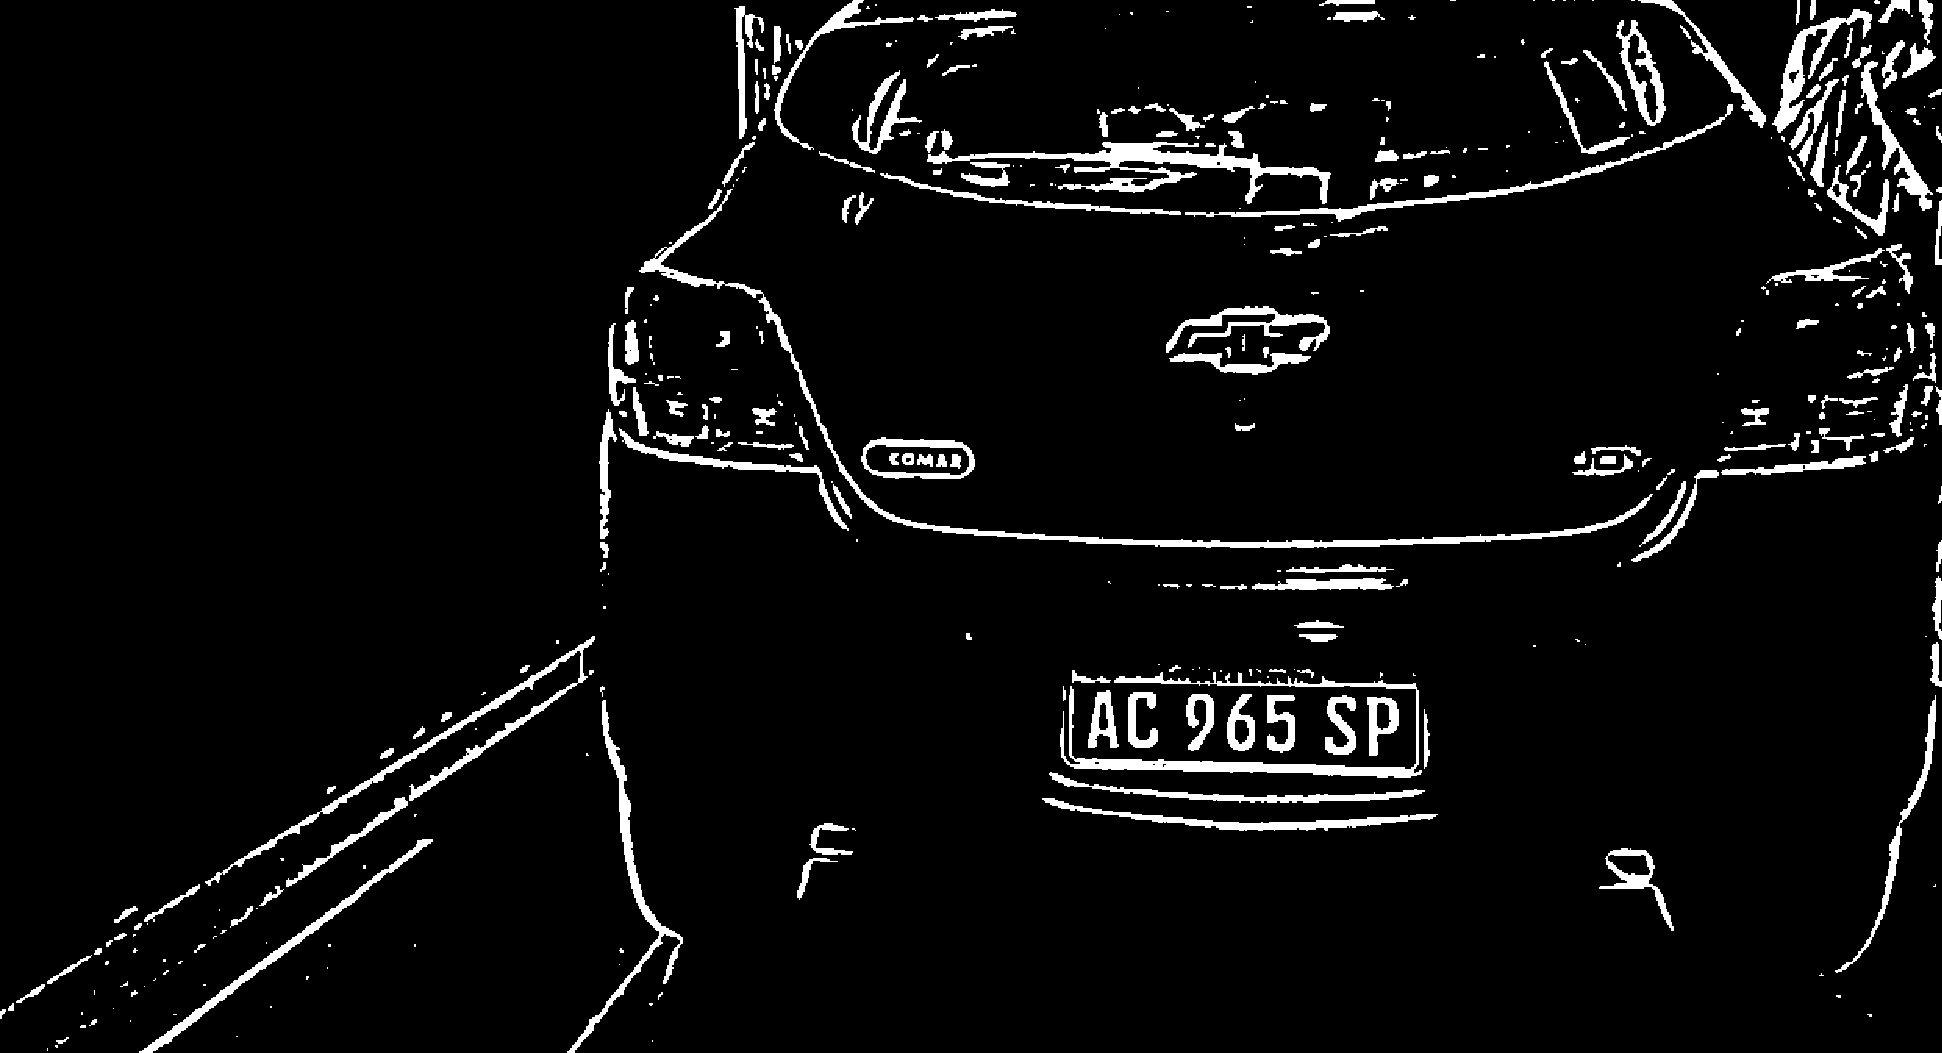
\includegraphics[scale=0.35]{imagen_binarizada.pdf}
	\caption{Imagen del vehículo que posee la patente a analizar,  luego de aplicarle el proceso de binarización.}
	\label{fig:img_bin}
\end{figure}
\begin{figure}[H]
	\centering
	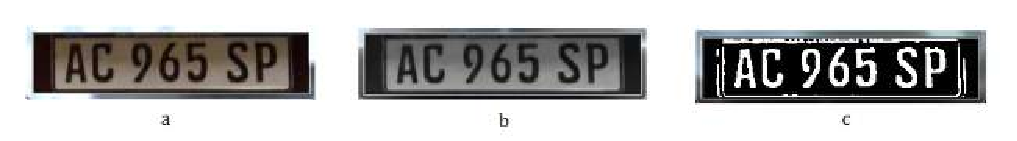
\includegraphics[width=\textwidth]{preprocesamiento_patente.pdf}
	\caption{Proceso de preprocesamiento de la región candidata: imagen original (a),  en escala de grises (b) y binarizada (c).}
	\label{fig:img_prepro}
\end{figure}


\noindent \textbf{Etapa 2: Segmentación de los caracteres de la patente}

En esta etapa, las diferentes imágenes que contienen patentes que son adquiridas por el sistema se redimensionan al mismo tamaño, de manera que el tamaño de los caracteres sea similar en todas ellas. El objetivo de esta fase es buscar las partes blancas de la imagen binarizada que cumplan con las especificaciones de los caracteres de la patente. Es por esto que en todo sistema ALPR se deben establecer algunos datos de las matriculas previamente para que el mismo quede configurado adecuadamente. Una vez que se detectan todos los caracteres de la placa, estos son aislados para luego identificarlos. El resultado del proceso de segmentación se observa en la figura~\ref{fig:img_segm}.

\begin{figure}[H]
	\centering
	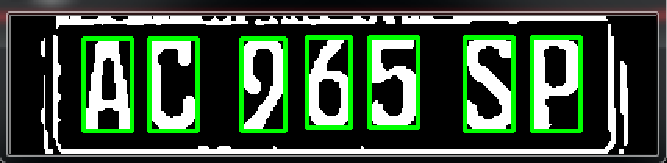
\includegraphics[scale=0.5]{segmentacion_caracteres.pdf}
	\caption{Resultado del proceso de segmentación de caracteres.}
	\label{fig:img_segm}
\end{figure}


\noindent \textbf{Etapa 3: Reconocimiento de los caracteres (OCR)}

Esta fase recibe los caracteres segmentados de la etapa anterior. Como su nombre lo indica, es la encargada de procesar cada uno de ellos y determinar a qué carácter alfanumérico corresponde. Para ello, pueden utilizarse numerosas herramientas de reconocimiento, tanto de software libre como de origen comercial, siendo la más conocida la llamada Tesseract OCR \cite{tesseractdoc}.

\quad

\noindent \textbf{Etapa 4: Post-procesamiento}

En algunos sistemas, el resultado de la etapa de reconocimiento no es solo la información obtenida del carácter analizado, sino que puede ser una lista de posibles valores con un porcentaje de confianza asociado a cada uno de ellos. En esta fase, el objetivo es tomar los resultados obtenidos y generar una lista de posibles resultados para las patentes, ordenándolas según el porcentaje de confianza. En caso de que el sistema no entregue una lista de posibilidades para los caracteres, solo se obtendrá un resultado. En la figura~\ref{fig:img_result}, se observa el resultado del proceso realizado por un sistema ALPR. Se muestra la imagen original junto con la cadena de caracteres que se corresponde con la patente.

\begin{figure}[H]
	\centering
	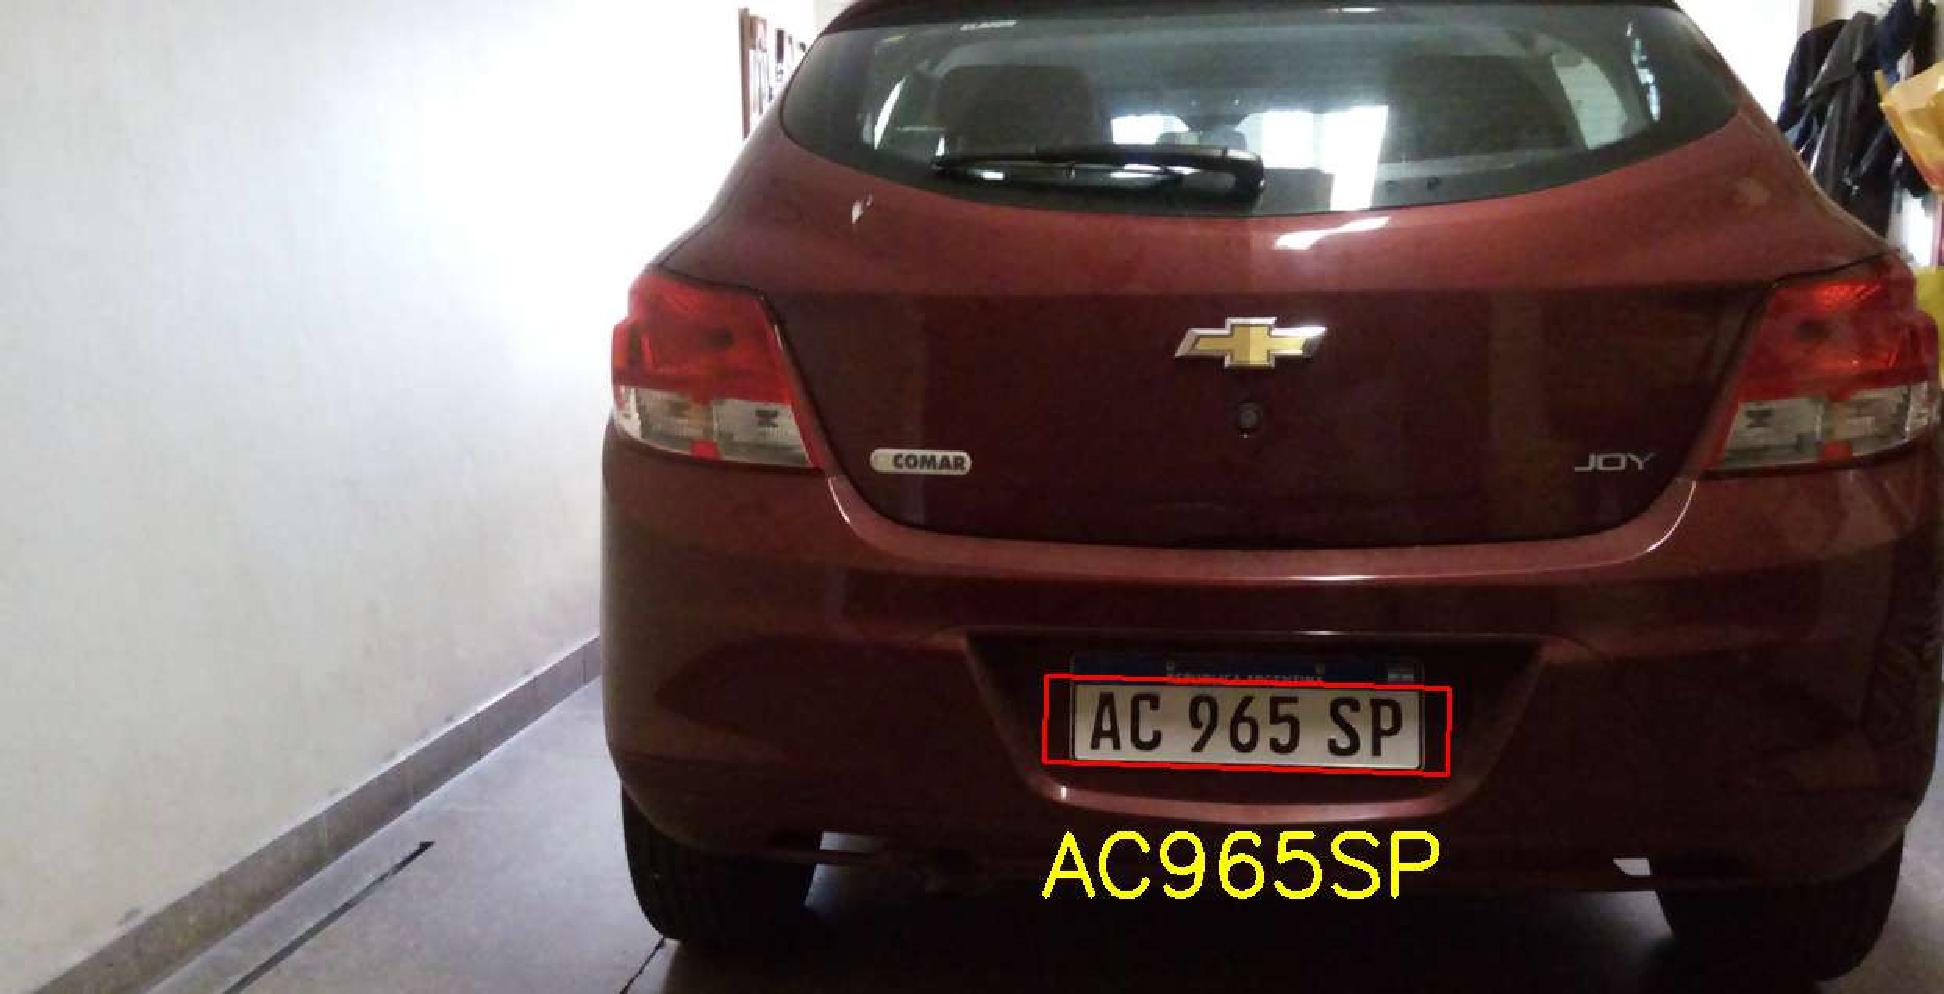
\includegraphics[scale=0.35]{resultado.pdf}
	\caption{Patente reconocida, resultante de la aplicación de un sistema ALPR.}
	\label{fig:img_result}
\end{figure}


\section{Descripción de las patentes y los conjuntos de datos}\label{sec:placpatarg}

\subsection{Patentes Argentinas} \label{key:patentesarg}

Actualmente, existen dos modelos de patentes que se encuentran en vigencia en el país \cite{Res-33-14-PATNT-MERCOSUR} \cite{caracpat1} \cite{caracpat2}.

\quad

\noindent \underline{\textbf{Patente del MERCOSUR}}

Las patentes del MERCOSUR poseen las características que pueden observarse en las figuras \ref{fig:img_pat1}, \ref{fig:img_pat2} y \ref{fig:img_pat3}, y que son listadas a continuación: 
\begin{itemize}
	\item Se implementa a partir del año 2016
	\item Está dotada de un arreglo de 7 caracteres que consta de letras y números y conforma un serial, embozado en alto relieve
	\item Elementos de seguridad que posee: 
	\begin{itemize}
		\item Bandera del país
		\item Emblema del MERCOSUR
		\item Marca de agua
		\item Tipo ensure 
		\item Estampado en caliente con lámina de seguridad con efecto difractivo y onda sinusoidal
	\end{itemize}
	\item Colores:
	\begin{itemize}
		\item Fondo de color blanco
		\item Caracteres de color negro
	\end{itemize}
	\item Dimensiones: 
	\begin{itemize}
		\item Vehículos:
		\begin{enumerate}
			\item Largo: 400mm $\pm$ 2mm
			\item Alto: 130mm $\pm$ 2mm
			\item Espesor: 1mm $\pm$ 0,2mm
		\end{enumerate}
		\item Motovehículos:
		\begin{enumerate}
			\item Largo: 200mm $\pm$  2mm
			\item Alto: 170mm $\pm$  2mm
			\item Espesor: 1mm $\pm$  0,2mm
		\end{enumerate}
	\end{itemize}
	\item Tipo de letra: 
	\begin{itemize}
		\item Fuente: FEEngschrift
		\item Alto del carácter en vehículos: 65mm 
		\item Alto del carácter en motovehículos: 53mm 
	\end{itemize}
\end{itemize}
\begin{figure}[H]
	\centering
	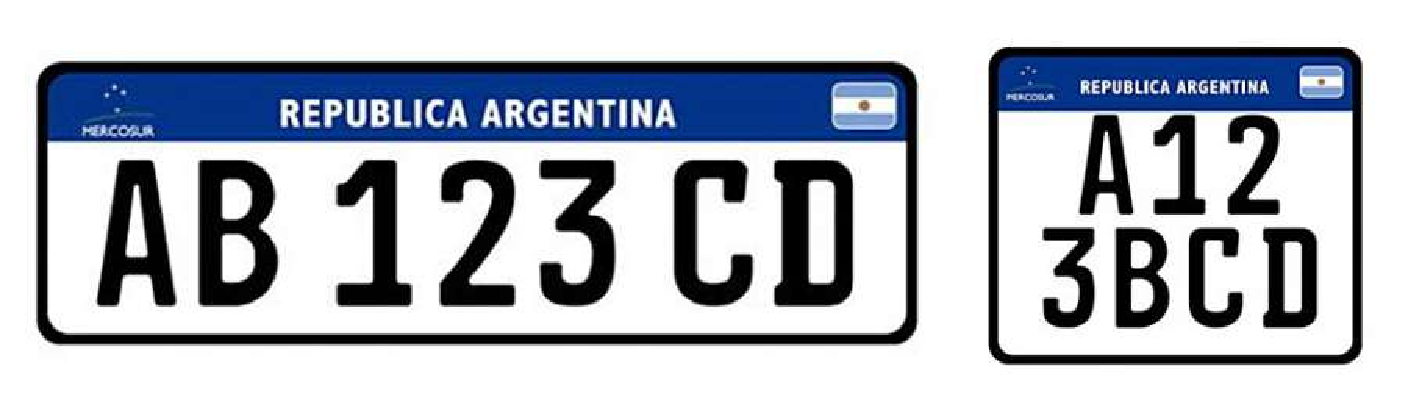
\includegraphics[scale=0.35]{pat1merc.pdf}
	\caption{Patente del MERCOSUR: características.}
	\label{fig:img_pat1}

	\quad

	\centering
	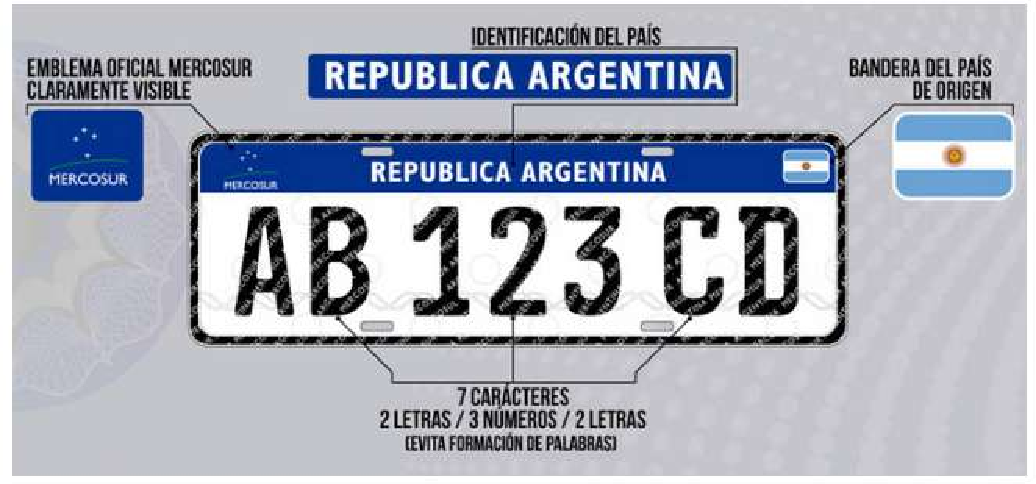
\includegraphics[scale=0.9]{pat2merc.pdf}
	\caption{Patente del MERCOSUR: medidas de seguridad.}
	\label{fig:img_pat2}
	
	\quad
	
	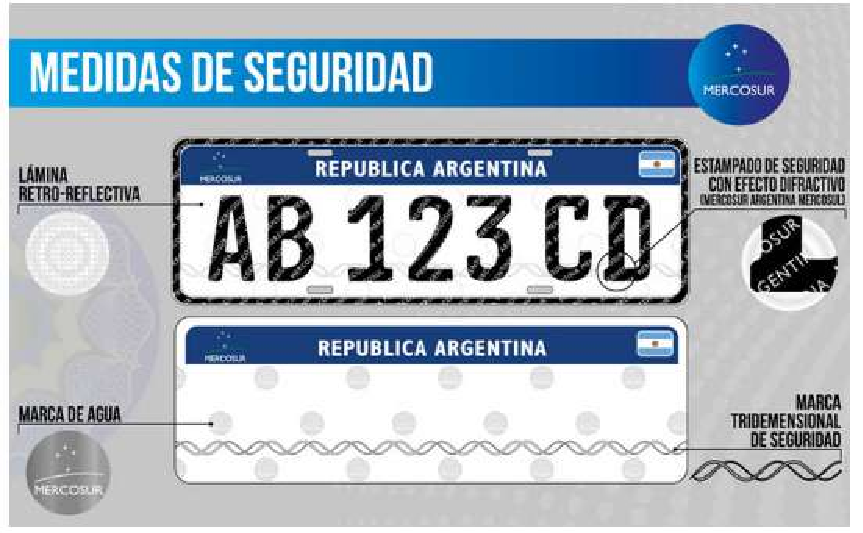
\includegraphics[scale=0.9]{pat3merc.pdf}
	\caption{Patente del MERCOSUR para automóviles y motocicletas.}
	\label{fig:img_pat3}
\end{figure}

\noindent \underline{\textbf{Patente argentina antigua}}

Las patentes antiguas poseen las características que pueden observarse en las figuras \ref{fig:img_pat1-2ant} y \ref{fig:img_pat3ant}, y que se listan a continuación: 

\begin{itemize}
	\item Se implementa entre el los años 1995 y 2016
	\item Está dotada de un arreglo de 6 caracteres que consta de letras y números y conforma un serial, embozado en bajo relieve
	\item Medidas de seguridad para evitar reproducción y/o adulteración que posee:
	\begin{itemize}
		\item Material de fabricación: aluminio
		\item Escudo Nacional a color, en el extremo superior izquierdo
		\item La palabra “ARGENTINA”, impresa en su parte media superior en color celeste
		\item Sellos circulares con la inscripción “RNPA” distribuidos en forma uniforme en los extremos blancos superior e inferior, los cuales pueden visualizarse haciendo variar la incidencia de luz sobre la misma. Se encuentran indicados en la figura~\ref{fig:img_pat1-2ant} con la letra (c)
		\item En caso de extravío, robo o hurto de la chapa patente, debe solicitarse una nueva. La única diferencia entre esta y la original es que la nueva, entre las letras y los números, lleva grabado en tamaño menor, pero de igual impresión, un carácter que determina la versión de la placa. Por ejemplo, “D” es de duplicado y  “T” es de triplicado, entre otros. Se encuentra indicado en la figura~\ref{fig:img_pat1-2ant} con la letra (d)
	\end{itemize}
	\item Colores:
	\begin{itemize}
		\item Banda central de color negro mate
		\item Caracteres sobre la banda central y de color blanco
		\item Bordes superior e inferior de color blanco reflectante
	\end{itemize}
	\item Dimensiones: 
	\begin{itemize}
		\item Vehículos:
		\begin{enumerate}
			\item Largo: 294mm 
			\item Alto: 129mm 
		\end{enumerate}
		\item Motovehículos:
		\begin{enumerate}
			\item Largo: 150mm 
			\item Alto: 130mm 
		\end{enumerate}
	\end{itemize}
%	\item Dimensiones: 
%	\begin{itemize}
%		\item Chapa metálica:
%		\begin{enumerate}
%			\item Largo: 294mm
%			\item Alto: 129mm
%		\end{enumerate}
%		\item Banda negra: 
%		\begin{enumerate}
%			\item Largo: 283mm
%			\item Alto: 78mm
%		\end{enumerate}
%	\end{itemize}
	\item Tipo de letra: 
	\begin{itemize}
		\item Fuente: LicensePlate 
		\item Ancho de los caracteres en vehículos: 32mm 
		\item Alto de los caracteres en vehículos: 67mm 
	\end{itemize}
\end{itemize}
\begin{figure}[H]
	\centering
	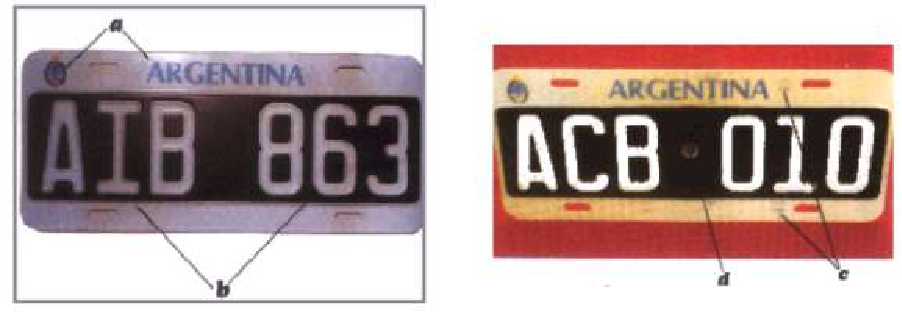
\includegraphics[width=\textwidth]{pat1-2ant.pdf}
	\caption{Patente argentina antigua correspondiente a automóviles.}
	\label{fig:img_pat1-2ant}
\end{figure}
\begin{figure}[H]
	\centering
	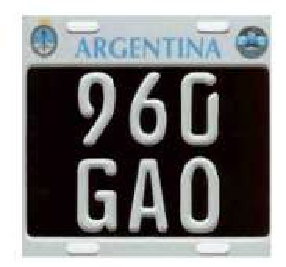
\includegraphics[scale=1]{pat3ant.pdf}
	\caption{Patente argentina antigua correspondiente a motovehículos.}
	\label{fig:img_pat3ant}
\end{figure}

A lo largo de esta sección, se plateó una numerosa lista de características correspondientes a cada uno de los modelos de patentes vigentes en nuestro país. Sin embargo, hay ciertos puntos que es necesario remarcar:
\begin{itemize}
	\item Mientras que las matrículas del MERCOSUR poseen caracteres negros sobre fondo blanco, en el modelo antiguo es a la inversa
	\item En las patentes nuevas, la letra “O” y el “0” son fácilmente diferenciables debido a que este último no se encuentra completo, debido a que posee un corte en la zona superior derecha 
	\item Respecto a las dimensiones de las mismas, el alto es similar en ambas. Sin embargo, el nuevo modelo es aproximadamente diez centímetros más ancha
	\item En cuanto a la calidad, debe mencionarse que las primeras patentes entregadas correspondientes al modelo del MERCOSUR tuvieron defectos de fabricación. Esto provocó la pérdida de pintura y el descoloramiento de las mismas \cite{fallaspat}
\end{itemize}


\subsection{Conjuntos de datos} \label{key:conjdatos}

Para probar el sistema OpenALPR y configurar sus parámetros de manera de obtener la mayor efectividad posible en su respuesta, se generaron dos conjuntos preliminares: un set de fotos para las patentes del Mercosur y otro para el modelo antiguo de matrículas argentinas. Ambos conjuntos están compuestos por 20 imágenes traseras de automóviles y camionetas. 

Esto se debe a que las motocicletas solo poseen patente en su parte trasera. Por otra parte, cabe destacar que el entorno de todas las imágenes es diferente, ya que no fueron tomadas en un mismo lugar. Por último, todas las fotos fueron tomadas con un smarthphone con una resolución de 4128 x 2322 pixeles, y luego se las re dimensionó a 1280x720 pixeles. Esta resolución se adoptó de manera de reducir el tiempo de procesamiento del sistema. La misma es configurable y admite modificaciones en caso de ser necesario. Estas imágenes fueron tomadas bajo estas condiciones, debido a que fueron pruebas preliminares y no se disponía aún de la cámara a utilizar.

Una vez finalizadas las pruebas de los diferentes parámetros del sistema, se decidió ampliar ambos sets de prueba a un tamaño de 165. Mediante estos dos nuevos conjuntos, se comprobó de mejor forma que los parámetros se hayan establecido correctamente. Las imágenes de estos sets fueron tomadas en condiciones que hacen que los mismos sean representativos del estacionamiento de prueba. Las imágenes se tomaron a distancias entre uno y cuatro metros respecto del vehículo, desde la parte trasera, a aproximadamente la altura de la matrícula, a vehículos que se encontraban detenidos y con condiciones de iluminación similares e incluso, en algunos casos, más complejas.

Por último, se crearon dos sets pequeños de 10 imágenes de motocicletas cada uno, para poder analizar el comportamiento del sistema para este tipo de vehículos.

Todos los conjuntos de imágenes establecidos, se detallan a continuación.

\subsubsection{Set de 20 imágenes de patentes del MERCOSUR}
Dentro de este conjunto, las imágenes poseen las siguientes características:
\begin{itemize}
	\item Todas las fotos son durante el día
	\item Nueve fotos fueron tomadas en línea recta a la patente y once desde un costado
	\item Se tomaron dos imágenes a un metro del vehículo, diecisiete a dos metros y una a tres metros de distancia aproximadamente
\end{itemize}

\subsubsection{Set de 20 imágenes de patentes antiguas}
Dentro de este conjunto, las imágenes poseen las siguientes características:
\begin{itemize}
	\item Todas las fotos son durante el día
	\item Once fotos fueron tomadas en línea recta a la patente y nueve desde un costado
	\item Se tomaron seis imágenes a un metro del vehículo, seis a dos metros y ocho a tres metros de distancia aproximadamente
\end{itemize}

\subsubsection{Set de 165 imágenes de patentes del MERCOSUR}
Dentro de este conjunto, las imágenes poseen las siguientes características:
\begin{itemize}
	\item Se tomaron 160 imágenes de día y 5 de noche
	\item 70 fotos fueron tomadas en línea recta a la patente y 95 desde un costado
	\item Se tomaron 33 imágenes a un metro del vehículo, 98 a dos metros, 33 a tres metros y una a cuatro metros de distancia aproximadamente
\end{itemize}

\subsubsection{Set de 165 imágenes de patentes antiguas}
Dentro de este conjunto, las imágenes poseen las siguientes características:
\begin{itemize}
	\item Se tomaron 160 imágenes de día y 5 de noche
	\item 82 fotos fueron tomadas en línea recta a la patente y 83 desde un costado
	\item Se tomaron 48 imágenes a un metro del vehículo, 90 a dos metros, 26 a tres metros y una a cuatro metros de distancia aproximadamente
\end{itemize}

\subsubsection{Set de 10 imágenes de motocicletas con patentes del MERCOSUR}
Dentro de este conjunto, las imágenes poseen las siguientes características:
\begin{itemize}
	\item Todas las fotos son durante el día
	\item 5 fotos fueron tomadas en línea recta a la patente y 5 desde un costado
	\item Se tomaron 3 imágenes a un metro del vehículo, 6 a dos metros y 1 a tres metros de distancia aproximadamente
\end{itemize}

\subsubsection{Set de 10 imágenes de motocicletas con patentes antiguas}
Dentro de este conjunto, las imágenes poseen las siguientes características:
\begin{itemize}
	\item Todas las fotos son durante el día
	\item 4 fotos fueron tomadas en línea recta a la patente y 6 desde un costado
	\item Se tomaron 4 imágenes a un metro del vehículo, 4 a dos metros y 2 a tres metros y de distancia aproximadamente
\end{itemize}


\section{Elección y ajuste del sistema para SAE}

El objetivo de esta sección, es presentar los diferentes tipos de software que se encuentran disponibles en la actualidad. Luego, se analizará el funcionamiento de dos de ellos en base a lo desarrollado en la sección \ref{key:conjdatos}, donde se explicó el funcionamiento general de un sistema ALPR. Estos sistemas fueron elegidos debido a que, al realizar una investigación sobre las herramientas disponibles, resultaron ser las que se encuentran más difundidas. Además, se expondrán los resultados de la experimentación realizada para ambos sistemas. Por último, se compararán ambos software, demostrando las razones por las que se decidió trabajar con la herramienta OpenALPR.

\subsection{Software disponibles} \label{key:implement}

Actualmente, existen numerosos trabajos realizados acerca del ALPR en los cuales cada autor lo aborda desde su perspectiva y aporta sus descubrimientos, problemáticas y resultados al investigar y experimentar con él.

Además, se tiene acceso a una gran cantidad de herramientas que permiten realizar el reconocimiento. Las mismas pueden ser sistemas pagos como “Anylines License Plate Scanner” \cite{anyline}, “Plate Recognizer” \cite{plate-recognizer} u “OpenALPR” \cite{openalpr}. En todos estos, no solo se ofrece la detección de patentes, sino que además se entregan otras funcionalidades como el almacenamiento y control en la nube, la posibilidad de integración a cualquier otro proyecto,  o bien una aplicación para smartphone, entre otras. 

Por otra parte, se pueden encontrar sistemas gratuitos, pero que no son de código abierto como lo es VISART \cite{visart}. Estos presentan la desventaja de que el proyecto se debe adaptar a lo que el software ofrece, debido a que este último no se puede modificar.

Por último, se pueden encontrar sistemas gratuitos de código abierto, entre los que podemos destacar “OpenCV 3 License Plate Recognition” \cite{opencv3}  y “OpenALPR” en su versión libre \cite{openalprfree}.

Todas estas herramientas tienen un principio de funcionamiento similar y deben ser adaptadas al lugar en el que se las pretende utilizar. Esto se debe a que las patentes de los diferentes países, estados o provincias pueden tener diversas fuentes, colores o estar escritas en distintos idiomas.

Por lo tanto, la ventaja de los sistemas pagos se encuentra en la gran variedad de países que contemplan para el reconocimiento. Pero, debido a que su uso implica una tarifa mensual o son muy costos, el desarrollo de este trabajo se focaliza en la utilización de un sistema gratuito de código abierto, el cual se busca adaptar inicialmente a las condiciones de las patentes argentinas y, a futuro, se ampliará a diferentes tipos de matrículas. Las opciones analizadas fueron ``OpenCV 3 License Plate Recognition'' y la versión libre de OpenALPR.

%Como se mencionó previamente en la sección \ref{sec:sysALPR}, hoy en día existe una gran cantidad de sistemas ALPR. Dentro de estos, se puede encontrar tanto software pago como gratuito (open source).
%En el primer grupo, se puede encontrar sistemas como “Anylines License Plate Scanner” \cite{anyline}, “Plate Recognizer” \cite{plate-recognizer} u “OpenALPR” \cite{openalpr}. En todos estos, no solo se ofrece la detección de patentes, sino que además se entregan otras funcionalidades como el almacenamiento y control en la nube, la posibilidad de integración a cualquier otro proyecto,  o bien una aplicación para smartphone, entre otras. 
%El segundo grupo está compuesto por desarrollos efectuados por terceros, como “OpenCV 3 License Plate Recognition Cpp” \cite{opencv3}, el cual es un sistema de reconocimiento de patentes basado en la librería OpenCV, realizado por Chris Dahms. Dentro de este grupo, también se puede encontrar sistemas pagos, los cuales presentan una versión de código abierto, para que diferentes desarrolladores puedan modificar el código y adaptarlo a sus necesidades, como es el caso de “OpenALPR” \cite{openalprfree}. Cabe destacar en este último caso, que este sistema no posee todas las funcionalidades de la versión comercial.
%El desarrollo de este trabajo se focalizará en la utilización de sistemas de código abierto, los cuales se buscará adaptar inicialmente a las condiciones de las patentes argentinas, y a futuro se ampliarán a diferentes tipos de matrículas. 
%En este caso, las opciones que se analizaron fueron las mencionadas anteriormente en el segundo grupo. Esto se debió a que, al realizar una investigación sobre el estado del arte, se concluyó que son las más utilizadas.

\subsection{Funcionamiento de los sistemas elegidos}\label{key:funcsistelegidos}

\subsubsection{OpenALPR}
Este es un software gratuito de código abierto, aunque también existe su versión comercial, utilizado para el reconocimiento automático de patentes de vehículos. OpenALPR está escrito en C++ y tiene la capacidad de analizar  imágenes fijas, videos y videos en tiempo real para identificar patentes en ellos y proveerla en forma de texto como salida \cite{openalprdoc}. 

Este sistema utiliza diferentes librerías para obtener el resultado, entre las que podemos destacar OpenCV \cite{libreriaopencv} para el procesamiento de la imagen y Tesseract \cite{tesseractdoc} para el reconocimiento de los caracteres.


\noindent \textbf{Etapas del sistema}	
	
Este sistema funciona bajo una arquitectura de tipo pipeline, es decir, consiste en ir transformando un flujo de datos secuencialmente a través de diferentes etapas. En este caso, la entrada del sistema es una imagen y la salida la patente del vehículo.
La documentación oficial \cite{developersguide} indica que, para obtener la respuesta, el software cuenta con 8 etapas, las cuales se comparan a continuación con las etapas generales de un sistema ALPR descriptas en la sección \ref{key:etapasgenerales}.

\quad

\noindent \textbf{Etapa 1: Detección de la patente}

Esta fase abarca las dos primeras etapas del OpenALPR que son la detección y la binarización. Esta fase funciona de la misma forma que se explicó para un sistema general, ya que se aplica un pre-procesamiento a la imagen para transformarla a escala de grises, y luego buscar la patente en dicha imagen. Para realizar esta búsqueda, el sistema utiliza un algoritmo denominado LBP (Local Binary Patterns) como algoritmo de detección.

Este es un operador de textura simple pero muy eficiente \cite{lbpalgoritmo}. Este algoritmo se encarga de extraer las características de la imagen, las cuales son lo que en visión artificial se denomina descriptores. El algoritmo, a partir de una imagen en escala de grises, calcula un valor para cada pixel de la imagen basándose en la vecindad de dicho pixel, es decir, en aquellos pixeles que lo rodean. Para hacer esto le otorga un 1 o un 0 a los pixeles de la vecindad si es que superan o no el valor del pixel central, para luego, a partir del valor binario generado, obtener el resultado LBP del pixel analizado pasando dicho valor a hexadecimal. Esto se puede observar en la figura \ref{fig:img_imagen_lbp}.

\begin{figure}[H]
	\centering
	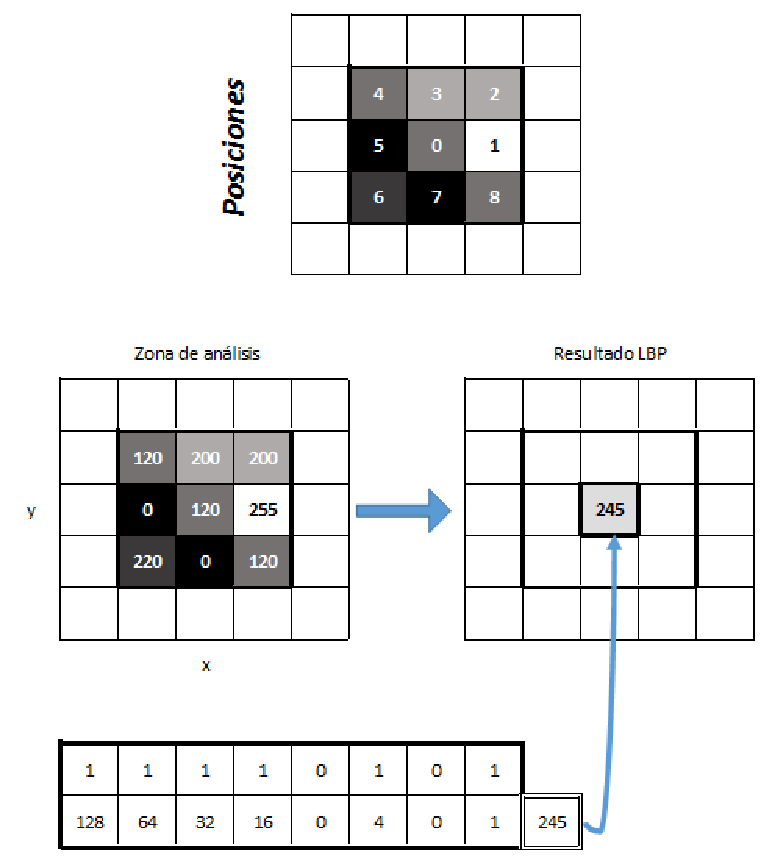
\includegraphics[scale=0.8]{imagen_lbp.pdf}
	\caption{Obtención del valor LBP de un pixel analizado \cite{imglbp}.}
	\label{fig:img_imagen_lbp}
\end{figure}

Cabe destacar que el pixel inicial puede ser cualquiera, siempre que se respete el mismo orden para todos. Luego, una vez obtenido el valor LBP para cada pixel, la parte de mayor importancia del método consiste en la generación de histogramas cuyos ejes poseen información del valor LBP de los pixeles y el porcentaje o cantidad de pixeles con ese valor.

Al obtener estos histogramas, el software OpenALPR es capaz de determinar la o las regiones donde los pixeles poseen un valor cercano a 255 (para el caso de patentes con fondo blanco) o a 0 (para patentes con fondo negro), que son los dos casos que acepta este sistema.Además, dichas regiones deben coincidir con las dimensiones preestablecidas para las patentes.

 De esta manera, el sistema es capaz de determinar la o las regiones de una o más posibles patentes en la imagen. Esto se observa en la figura \ref{fig:img_pos_pat}, donde los rectángulos de color rojo son el resultado de esta primera etapa. 	

\begin{figure}[H]
	\centering
	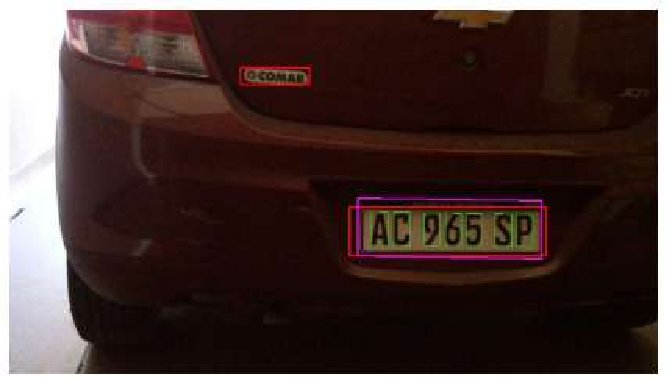
\includegraphics[scale=1]{alpr_posPat.pdf}
	\caption{Posibles patentes detectadas.}
	\label{fig:img_pos_pat}
\end{figure}

Por último, se toma un recorte de la patente de la imagen en escala de grises y se la binariza para luego ser tratada en las siguientes etapas. Cabe destacar que el sistema crea múltiples imágenes binarizadas para evitar la pérdida de un carácter en el caso de una imagen muy brillante u oscura. Para realizar la binarización, este sistema utiliza los métodos de Wolf-Jolion \cite{wolf2004} y Sauvola \cite{adaptive-document-binarization}. El método de Wolf-Jolion propone un sistema para la localización, mejora y binarización del texto en documentos multimedia. En este caso, la detección se realiza aplicando una medida de gradientes acumulados, los cuales se suelen binarizar con el método de Otsu \cite{revistaiberoamericana}. En este caso, el sistema utiliza el método Sauvola en lugar del de Otsu. El mismo aplica una ecuación de binarización de cálculo, a partir de un umbral, y utilizando la media, el nivel de desviación y la intensidad de los pixeles de la imagen. Si bien este algoritmo es más lento que el de Otsu, en imágenes con grises muy sutiles y degradados, proporciona resultados mucho más nítidos, más claros y limpios\cite{rmagro}.

\quad

\noindent \textbf{Etapa 2: Segmentación de caracteres}

 En OpenALPR esta fase abarca cuatro etapas: el análisis de caracteres, la detección de bordes de la patente, el enderezamiento y la segmentación de caracteres. En este caso, el sistema no recurre a aislar los caracteres directamente, sino que efectúa un procedimiento previo para lograr obtener mejores resultados en el reconocimiento.

En primer lugar, se buscan en las imágenes binarizadas todas las manchas que coincidan con el alto y ancho establecidos para los caracteres de la patente, tal como se observa en la figura~\ref{fig:img_det_analys}.

\begin{figure}[H]
	\centering
	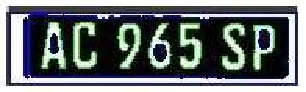
\includegraphics[scale=1]{alpr_det_analys.pdf}
	\caption{Detección y análisis de los posibles caracteres.}
	\label{fig:img_det_analys}
\end{figure}

Una vez ubicados los caracteres, se utiliza el algoritmo de Canny combinado con la transformada de Hough. Mientras el primero permite localizar contornos en la imagen, el segundo se usa para encontrar objetos en una imagen, tales como rectas, circunferencias o eclipses \cite{navacerrada}.

El objetivo de la aplicación de estos algoritmos es detectar los bordes de la patente para luego realizar el enderezamiento de la imagen y segmentar los caracteres de forma más eficiente. Este resultado, se puede observar en las figuras ~\ref{fig:img_det_bordes}(a), ~\ref{fig:img_det_bordes}(b) y ~\ref{fig:img_det_bordes}(c) donde se pueden ver las líneas ganadoras, tanto verticales como horizontales, luego de aplicar la transformada de Hough.

\begin{figure}[H]
	\centering
	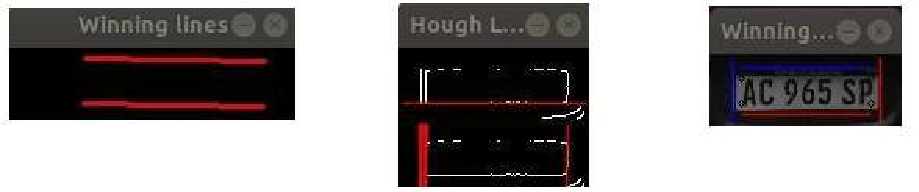
\includegraphics[width=\textwidth]{alpr_detBordes.pdf}
	\caption{Detección de bordes horizontales (a) y verticales (b), y detección de patente (c).}
	\label{fig:img_det_bordes}
\end{figure}

Por último, para segmentar los caracteres, se utiliza un histograma vertical para encontrar los espacios entre los caracteres de la patente, lo que permite leer y procesar cada carácter por separado. Además, esta etapa se encarga de limpiar los caracteres al remover puntos desconectados, descalificar regiones de caracteres por ser muy chicas e intenta remover los bordes de la patente, de manera de que no sean calificados como un “1” o una “I”. El resultado de todos estos procesos es el que se visualiza en la figura~\ref{fig:img_char_limp}.

\begin{figure}[H]
	\centering
	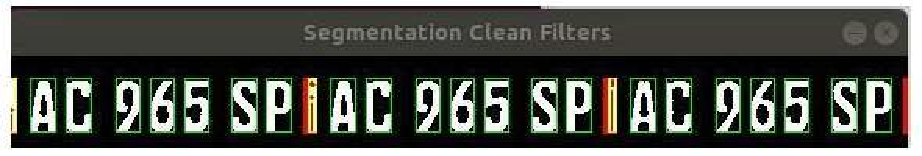
\includegraphics[width=\textwidth]{alpr_char_limp.pdf}
	\caption{Caracteres limpios y segmentados.}
	\label{fig:img_char_limp}
\end{figure}

\quad

\noindent \textbf{Etapa 3: Reconocimiento de caracteres}

Esta etapa de reconocimiento de caracteres se corresponde con la séptima etapa de OpenALPR, que lleva el mismo nombre. La misma no presenta ninguna diferencia con lo explicado en la etapa general, ya que reconoce los caracteres y, para cada uno de ellos, entrega todas las posibilidades que hay junto a un porcentaje de confianza.

Como motor de OCR, este software utiliza Tesseract. Esta herramienta se encarga, en primer lugar, de almacenar los contornos pertenecientes a los objetos de la imagen binaria que se le aporta. Luego, dichos objetos son ordenados en diferentes líneas de texto según la ubicación dentro de la imagen (coordenadas X,Y) de los contornos almacenados. Estas líneas, ahora son divididas en palabras, donde si los caracteres de esta presentan un ancho de separación fijo, cada uno de ellos se introduce en una celda de carácter. En caso contrario se divide únicamente en palabras según valores de espaciado entre ellas predefinidos.

A partir de este momento, el proceso entra en dos fases. En la primera de ellas, se hace un intento por reconocer, mediante un clasificador, cada una de las palabras (o carácter) que conforman el texto. Las que se reconocen positivamente se pasan a un clasificador adaptativo como patrón de entrenamiento, consiguiendo mayor capacidad de acierto al avanzar en el análisis del texto.

La segunda fase consiste en una nueva revisión del texto para intentar reconocer las palabras o caracteres en las que se haya fallado en la primera fase. Esto se hace debido a que el clasificado fue mejorado con los resultados positivos de la primera fase \cite{politecnicacartagena}.

Una parte de esta etapa se puede visualizar en el fragmento de la figura~\ref{fig:img_rec_char}.

\begin{figure}[H]
	\centering
	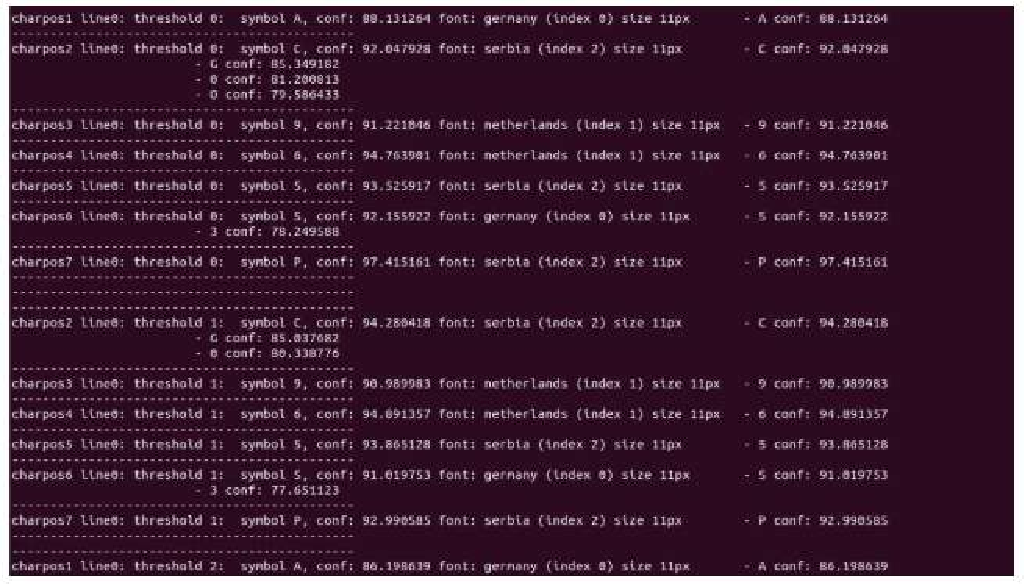
\includegraphics[width=\textwidth]{alpr_recChar.pdf}
	\caption{Fragmento del proceso de reconocimiento de los caracteres.}
	\label{fig:img_rec_char}
\end{figure}


\noindent \textbf{Etapa 4: Post-procesamiento}

Corresponde a la etapa final de este sistema y lleva el mismo nombre que la última de las etapas generales mencionada en la sección \ref{key:etapasgenerales}. En esta instancia se establece un umbral, que es un puntaje que el software calcula para el carácter basándose en la confianza y las ocurrencias de dicho carácter al reconocer los caracteres de las múltiples imágenes binarias que se generan. Entonces, si el valor resultante del carácter se encuentra por debajo del umbral, este queda rechazado como posibilidad y se lo descarta.

Luego, el sistema se encarga de determinar la mejor combinación de los resultados positivos, entregando una lista de posibles patentes ordenándolas de mejor a peor según su confianza. Esta lista, es generada a partir de permutaciones entre las posibilidades que son válidas para cada carácter. Cabe destacar que el número de patentes presente en la misma se puede seleccionar, sabiendo que no siempre se va a obtener esa cantidad máxima. 

Por último, esta etapa posee la capacidad de validar el formato de las combinaciones que se obtienen. Esto hace referencia a que se le puede decir al sistema que la patente es de determinada forma (por ejemplo: [letra][letra][letra]-[numero][numero][numero]) para que el mismo entregue solo respuestas que coincidan con dicha forma. De esta manera, se evitan las posibles confusiones entre letras y números, ya que si se reconoce un numero donde se estableció que debía haber una letra, ese resultado queda inmediatamente descartado.
El resultado final se puede observar en la figura~\ref{fig:img_postpro}. 

\begin{figure}[H]
	\centering
	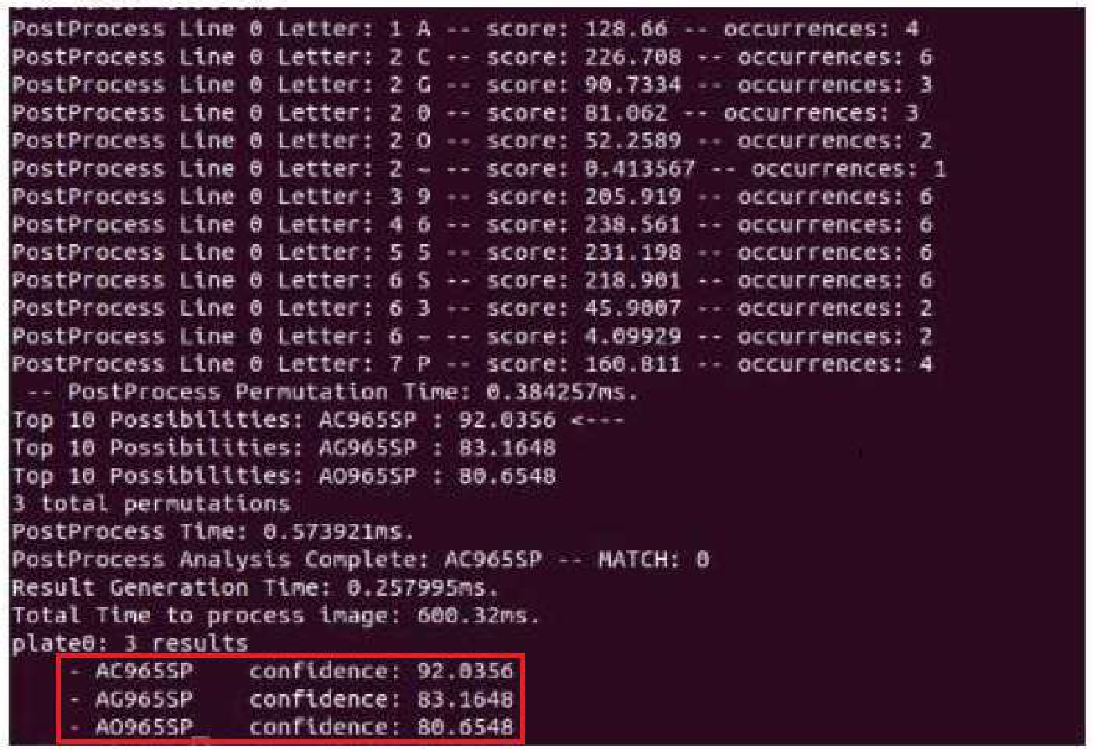
\includegraphics[width=\textwidth]{alpr_postpro.pdf}
	\caption{Fragmento de la etapa de postprocesamiento junto con el listado de patentes obtenido como resultado del proceso completo.}
	\label{fig:img_postpro}
\end{figure}


\noindent \textbf{Opciones de funcionamiento del sistema}

El software OpenALPR es capaz de reconocer matrículas a partir de tres diferentes fuentes: imágenes fijas, videos o videos en tiempo real. Cabe destacar que el proceso de obtención de la patente es idéntico para los tres casos. Esto se debe a que, en el caso de los videos, lo que se hace es analizar los diferentes frames del mismo para encontrar la patente. Es decir, el análisis se realiza a partir de una imagen que se extrae del video. 

Luego de evaluar las tres posibilidades para este proyecto, se considera más apropiado y sencillo utilizar el video en tiempo real. Esto se debe a que el sistema permanecerá continuamente analizando el video para encontrar una patente. En el caso de las imágenes fijas, primero se debería determinar el momento en que se realizaría la captura de la imagen, lo que implicaría el desarrollo de un código externo para ello. Luego, se la utilizaría para realizar el reconocimiento. Para los videos, la situación es similar. Sin embargo, se debería determinar cuándo comenzar y finalizar el video.  Además, este proceso es mucho más costoso computacionalmente y, por ende, se demora más tiempo en obtener una respuesta.

Por último, la principal ventaja de trabajar con video en lugar de imágenes fijas es que al estar continuamente analizando los frames del mismo, el sistema es capaz de entregar la respuesta para una misma patente varias veces. De esta manera, es posible obtener un resultado con mayor nivel de confianza. Para lograr esto con imágenes, se deberían obtener varias por vehículo y analizar cada una de ellas. Esto aumentaría los recursos computacionales requeridos. 

Por estos motivos, se determinó que la mejor opción es trabajar a partir del video en tiempo real. Para ello, el sistema cuenta con un modo de funcionamiento denominado alprd (alpr daemon) el cual funciona en segundo plano y permite entregarle al sistema un stream de vídeo en tiempo real.

Cuando el sistema detecta una matrícula en el vídeo, procesa el frame. A partir del mismo se obtiene el número de la patente junto con su confianza, y algunas características adicionales como el tiempo de procesamiento, la ubicación de la patente en la imagen, entre otras.

Una vez obtenida dicha información, el sistema tiene dos formas de seguir adelante. En la primera de ellas, esta es enviada a una cola de trabajo y luego a un servidor HTTP, del cual se pueden extraer los datos que contiene. La segunda forma, que es la implementada en este proyecto, es utilizando únicamente la cola de trabajo. En este caso, la misma funciona bajo el protocolo Beanstalk. Este es un protocolo que corre sobre TCP y se encarga de crear un servidor web al que el sistema sube el resultado como un nuevo trabajo o Job \cite{beanstalkprotocol}.

Para recuperar la información contenida dentro de los trabajos, es necesario extraer a estos últimos de la cola. Para ello, se usa un consumidor de cola. En este caso, para realizar esto, se desarrolló un código en C++ (podría ser en otro lenguaje) al que se añadió la librería Beanstalk-client para utilizar algunas de sus funciones con el objetivo de conectarse a este servidor, seleccionar la cola a usar, reservar un trabajo, entre otras \cite{beanstalkclient}.

Finalmente, la información recuperada se encuentra en formato “.Json”. De esta manera, a partir de un código se puede acceder fácilmente a las diferentes secciones de la misma, pero al extraer los trabajos mediante el mismo, esta pierde el formato y como resultado se obtiene una cadena de caracteres. Por lo tanto, para evitar tener que buscar la información deseada (como la patente obtenida o la confianza) en dicho texto sin formato, se dota al código de C++ de otra librería. La misma permite llevar todo ese texto al formato original (“. Json”) y trabajar con el mismo en C++ \cite{jsoncons}.

De esta manera, el sistema es capaz de obtener la información de la patente del vehículo que se ha posicionado delante de la cámara \cite{alprd}. 



\subsubsection{OpenCV 3 License Plate Recognition}
El mismo es un programa de código abierto desarrollado por Chris Damhs, el cual está implementado sobre el lenguaje C++ y está basado en la utilización de la librería OpenCV \cite{libreriaopencv}.

Este sistema tiene una estructura tipo pipeline, ya que se atraviesan diferentes etapas para lograr obtener la patente del vehículo deseado.

Respecto a la etapa general inicial de los sistemas ALPR, este software se diferencia en que, en lugar de buscar la patente en la imagen, busca primero posibles caracteres de esta para luego ubicarla. Para realizar esto, aplica en primera instancia un pre-procesamiento sobre la imagen en el que se la transforma a escala de grises y luego se la binariza mediante la función AdaptativeThresh. La misma usa binarización Gaussiana. Los resultados parciales de este proceso pueden observarse en las figuras \ref{fig:img_orig_opencv}, \ref{fig:img_escGrey_opencv} y \ref{fig:img_bin_opencv}.

\begin{figure}[H]
	\centering
	\begin{subfigure}[b]{0.49\textwidth}
		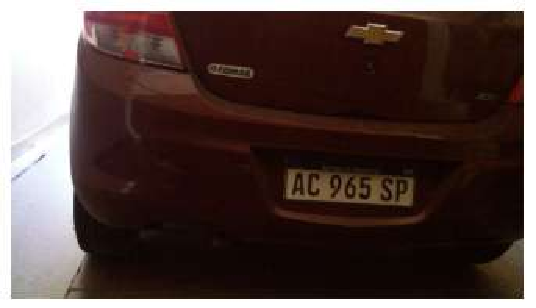
\includegraphics[width=\textwidth]{openCV_imagen_original.pdf}
		\caption{Imagen original.}
		\label{fig:img_orig_opencv}
	\end{subfigure}
	\hfill
	\begin{subfigure}[b]{0.49\textwidth}
		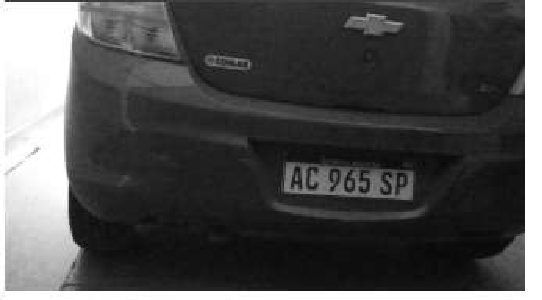
\includegraphics[width=\textwidth]{openCV_imagen_escgrises.pdf}
		\caption{Imagen en escala de grises.}
		\label{fig:img_escGrey_opencv}
	\end{subfigure}
	\hfill
	\begin{subfigure}[b]{0.49\textwidth}
		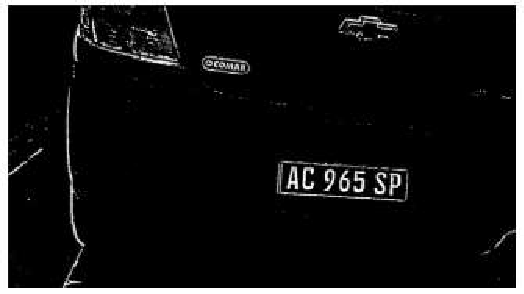
\includegraphics[width=\textwidth]{openCV_imagen_binarizada.pdf}
		\caption{Imagen binarizada.}
		\label{fig:img_bin_opencv}
	\end{subfigure}
	\caption{Resultados parciales de la etapa inicial del software basado en OpenCV.}
\end{figure}

Una vez que la imagen se encuentra binarizada se procede a buscar todos los contornos dentro de la misma. Luego, se eliminan aquellos que no coincidan con las dimensiones establecidas para los caracteres. Esto se puede observar en las figuras~\ref{fig:img_cont_opencv} y~\ref{fig:img_caract_opencv}.

\begin{figure}[H]
	\centering
	\begin{subfigure}[b]{0.49\textwidth}
		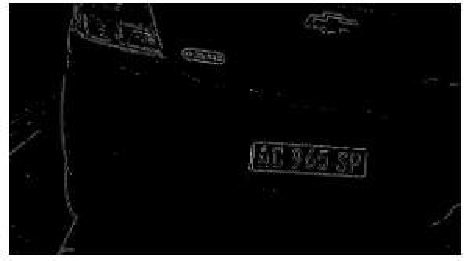
\includegraphics[scale=1]{openCV_imagen_contornos.pdf}
		\caption{Contornos dentro de la imagen binarizada.}
		\label{fig:img_cont_opencv}
	\end{subfigure}
	\hfill
	\begin{subfigure}[b]{0.49\textwidth}
		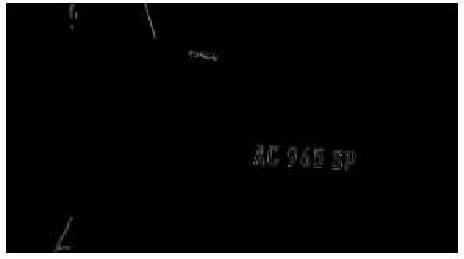
\includegraphics[scale=1]{openCV_imagen_caracteres.pdf}
		\caption{Caracteres que superaron el proceso de eliminación.}
		\label{fig:img_caract_opencv}
	\end{subfigure}
	\caption{Proceso de búsqueda de contornos y eliminación de aquellos que no poseen dimensiones de caracteres.}
\end{figure}

Con estos contornos, el sistema procede a generar diferentes grupos de caracteres, los cuales poseen características similares entre sí como el tamaño y la ubicación en las fotos. Si el grupo generado no posee un mínimo de caracteres preestablecido, queda descartado. Este resultado se observa en la figura~\ref{fig:img_caract_coinc_opencv}.

\begin{figure}[H]
	\centering
	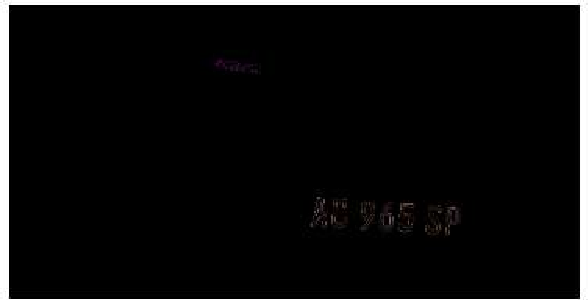
\includegraphics[scale=1]{openCV_imagen_caractCoincident.pdf}
	\caption{Grupos de caracteres coincidentes.}
	\label{fig:img_caract_coinc_opencv}
\end{figure}

Por último, basándose en la ubicación de los caracteres, el sistema los ordena y realiza un recorte de la región donde se encuentra el grupo en la imagen original. Por lo tanto, en la etapa de detección de patente, este software no entrega la ubicación de la matrícula en la imagen, sino que entrega un conjunto de posibles patentes, a las cuales se les aplica el mismo pre-procesamiento que a la imagen original, es decir, se lleva a escala de grises y se las binariza. Esto se ve en las figuras~\ref{fig:img_patente-correcta},~\ref{fig:img_patente-incorrecta} y ~\ref{fig:img_patente-luego-preproc}.

\begin{figure}[H]
	\centering
	\begin{subfigure}[b]{0.49\textwidth}
		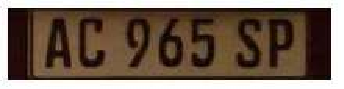
\includegraphics[width=\textwidth]{Patente-correcta.pdf}
		\caption{Patente correcta.}
		\label{fig:img_patente-correcta}
	\end{subfigure}
	\hfill
	\begin{subfigure}[b]{0.49\textwidth}
		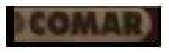
\includegraphics[width=\textwidth]{Patente-incorrecta.pdf}
		\caption{Patente incorrecta.}
		\label{fig:img_patente-incorrecta}
	\end{subfigure}
	\hfill
	\begin{subfigure}[b]{0.49\textwidth}
		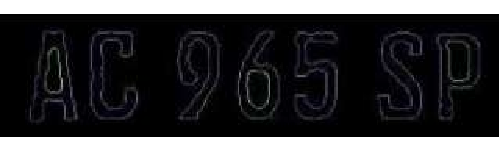
\includegraphics[scale=1]{Patente-luego-preproc.pdf}
		\caption{Patente resultante luego de aplicar el pre-procesamiento.}
		\label{fig:img_patente-luego-preproc}
	\end{subfigure}
	\caption{Proceso desarrollado en la etapa de detección de patente.}
\end{figure}

Siguiendo con el esquema general de los sistemas ALPR, esta herramienta busca segmentar los caracteres de las posibles patentes que se hayan encontrado. Para esto, realiza el mismo procedimiento utilizado para encontrar caracteres en la imagen original, pero ahora sobre la imagen de la posible patente. Una vez encontrados, mediante una comparación de tamaños y ubicación, se remueven los caracteres internos (círculo interior dentro del ``0'' o la ``O'') o superpuestos, que pueden ser considerados como un carácter diferente por sus dimensiones. De esta manera, se evita incluir dos veces el mismo carácter o caracteres extra. La figura ~\ref{fig:img_caract_remov_opencv} muestra el resultado de esta etapa.

\begin{figure}[H]
	\centering
	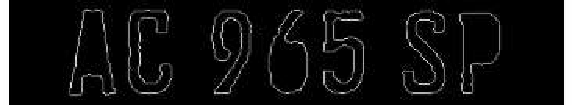
\includegraphics[scale=1]{openCV_imagen_caractIntRemov.pdf}
	\caption{Resultado de la remoción de caracteres internos.}
	\label{fig:img_caract_remov_opencv}
\end{figure}

En la fase de reconocimiento de caracteres (tercera etapa general de los sistemas ALPR) este software presenta falencias ya que, en primer lugar, solo aplica el reconocimiento a la posible patente que contenga un mayor número de caracteres. Esto lo hace muy sensible a variaciones en el entorno de la imagen. En segundo lugar, utiliza el algoritmo K-NN (K Nearest Neighbours) \cite{MEMORIA-ARCEARROYO}  el cual, si bien es capaz de entregar una respuesta, no es un motor de OCR. Este es uno de los algoritmos supervisados más simples de Machine Learning, el cual se usa mayormente para la clasificación. Básicamente determina a que grupo pertenece un nuevo elemento dependiendo de cómo están clasificados sus vecinos más cercanos. Es decir, almacena todos los casos conocidos que se poseen y los utiliza para clasificar nuevos casos dependiendo de la similitud que tenga con las características determinadas \cite{navacerrada}.

Por último, se encuentra la fase de post-procesamiento. En esta, el sistema toma el resultado obtenido para cada uno de los caracteres, los cuales fueron ordenados previamente, e informa el resultado marcando con un recuadro rojo la patente seleccionada. Junto a ella, coloca los valores de los caracteres. Este último proceso se puede observar la la figura  ~\ref{fig:img_result_opencv}.

\begin{figure}[H]
	\centering
	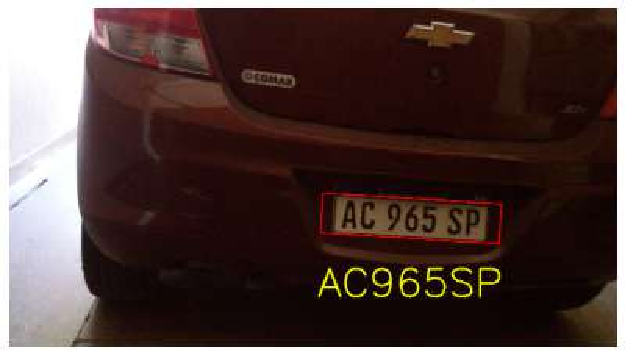
\includegraphics[scale=1]{openCV_imagen_resultado.pdf}
	\caption{Resultado entregado por la fase de post-procesamiento.}
	\label{fig:img_result_opencv}
\end{figure}	
		
		
\subsection{Experimentación y puesta a punto de los sistemas} \label{key:experimentaconypuesta}
	
En esta sección se desarrollarán las modificaciones realizadas sobre cada uno de los sistemas trabajados, con el objetivo de mejorar los resultados devueltos por ellos. Además, podrá observarse el impacto provocado por las mismas, al visualizar las respuestas obtenidas antes y después de modificar dichos sistemas. 

Para evaluar el funcionamiento de estos sistemas, se utilizó un ordenador con sistema operativo Ubuntu 18.04 LTS, un procesador Intel Core I5 de segunda generación con cuatro núcleos y 4GB de memoria RAM. 

		
\subsubsection{OpenALPR}		
		
Inicialmente, se utilizaron los sets de 20 imágenes, descritos en la sección \ref{key:conjdatos}, para evaluar el sistema con sus parámetros por defecto. Los resultados de esta prueba se muestran en la tabla \ref{tabla:openalpr_Torig}, donde en la columna ``='' se muestran las patentes reconocidas correctamente, en la columna ``X'' aquellas que fueron detectadas por el sistema con algún error en uno o más de sus caracteres y, por último, en la columna ``NF'', se encuentran las imágenes en las que el sistema no detectó ninguna patente. Esta simbología se mantendrá a lo largo de la sección de experimentación.
		
\begin{table}[htbp]
	\begin{center}
		\begin{tabular}{|c|c|c|c|}
			\hline
			& \multicolumn{3}{c|}{Set de 20 imágenes}\\
			\hline
			MERCOSUR & 75\% (15) & 10\% (2) & 15\% (3)\\
			\hline 
			Antiguas & 40\% (8) & 5\% (1) & 55\% (11)\\ \hline
		\end{tabular}
		\caption{Resultados de la detección con el entrenamiento original.}
		\label{tabla:openalpr_Torig}
	\end{center}
\end{table}		
		
Para mejorar el rendimiento de este software, fue necesario adaptarlo a las patentes argentinas. Para ello, se crearon diferentes archivos, los cuales se describen a continuación:	
		
\begin{enumerate}
	\item \textbf{\underline{Archivos de configuración de las patentes:}}
	
	A partir de lo expuesto en la sección \ref{key:patentesarg}, se crearon dos archivos de configuración (archivos de extensión ``.conf''), uno para las patentes del MERCOSUR y otro para el modelo antiguo. Dentro de estos archivos, se configuraron las dimensiones de cada una de las placas: alto, ancho, tamaño de los caracteres, entre otros. Además, se estableció la cantidad máxima y mínima de caracteres que debe poseer cada patente: 7 para modelo MERCOSUR y 6 para el antiguo. Por otra parte, el software está preparado por defecto para leer letras negras sobre un fondo blanco. Sin embargo, trabajando sobre estos archivos es posible invertir los colores de la patente para poder leer letras blancas sobre un fondo negro. Esto último se realizó únicamente en el archivo de las patentes antiguas. Adicionalmente, en estos archivos se debe configurar el entrenamiento que se aplica al motor de OCR, y el archivo del detector a utilizar. 
	
	Luego, debido a las similitudes que presentan las dimensiones de las patentes del MERCOSUR con respecto a las de las matriculas europeas, se decidió establecer estos parámetros en forma coincidente con los correspondientes a esta región, los cuales ya forman parte de la versión de código abierto de este software. En el caso del modelo antiguo ocurre algo similar con respecto a las matrículas estadounidenses, por lo que se procede de la misma forma que en el caso anterior. Por último, cabe destacar que el resto de los parámetros que se deben establecer mantuvieron los valores correspondientes a los de las matriculas europeas y estadounidenses, respectivamente.
	
	\item \textbf{\underline{Archivos de Post-Procesamiento:}}
	
	Como se mencionó en la sección \ref{key:funcsistelegidos}, el sistema es capaz de validar el formato de las combinaciones que se forman. Para realizar esto, el software utiliza, para cada estilo de patente que posee, un archivo de extensión ``.patterns'', en el cual se indica el o los formatos posibles de cada patente. Por lo tanto, se creó un archivo para las patentes del MERCOSUR donde se estableció el formato @@ \#\#\# @@, donde @ representa las letras  y \# los números. 
	
	Por otra parte, se debe destacar que en este archivo se pueden agregar los formatos del resto de las patentes del MERCOSUR, de forma de poder reconocerlas, ya que las dimensiones son las mismas. Finalmente, para las patentes argentinas antiguas se creó otro archivo en el que se estableció el formato @@@ \#\#\#.
	
	\item \textbf{\underline{Openalpr.defaults.conf:}}
	
	Es el archivo de configuración general del sistema. Contiene los parámetros por defecto establecidos en el sistema. Con el objetivo de mejorar el funcionamiento del mismo en el caso de las patentes argentinas se modificaron algunos de estos valores. Entre ellos, podemos destacar los siguientes:
	\begin{itemize}
		\item \textbf{detection\_iteration\_increase}
		
		Por defecto, este valor está establecido en 1.1.  Sin embargo, por los resultados obtenidos en la experimentación, se considera que el valor 1.07 es el que otorga mejores resultados. Cabe destacar, que este parámetro es el porcentaje de incremento del cuadro del algoritmo LBP para cada iteración, donde cuanto más bajo es su valor, más lento es el sistema.
		
		\item \textbf{must\_match\_pattern}	
		
		Este valor por defecto es 0. Su función al tomar el valor uno es informarle al sistema que las respuestas que otorgue deben coincidir con los formatos establecidos en los archivos de post-procesamiento y, en caso contrario, descartarla. Se lo seteó en 1.
		
		\item \textbf{postprocess\_min\_confidence}	
		
		Por defecto, este parámetro está establecido en 65. Este valor determina el mínimo de confianza que debe poseer cada símbolo luego de pasar por el OCR para ser considerado. Se decidió disminuirlo a 55, debido a que en este valor se obtenían una mayor cantidad de respuestas correctas que con el valor por defecto.
		
		\item \textbf{detection\_mask\_image}	
		
		Por defecto este parámetro está vacío, lo que significa que el sistema debe analizar toda la imagen en busca de la patente. Al establecer una máscara, como se observa en la figura~\ref{fig:img_mask}, el sistema solo analizará las partes blancas de la imagen e ignorará las partes negras, generando un resultado más veloz. De esta forma, se logra reducir el tiempo de procesamiento del algoritmo LBP, disminuyendo el tiempo total de procesamiento en aproximadamente 30\% con una máscara como la de la figura~\ref{fig:img_mask}. Cabe aclarar que el tiempo que se reduzca depende de la forma que posea la máscara.
		
		\begin{figure}[H]
			\centering
			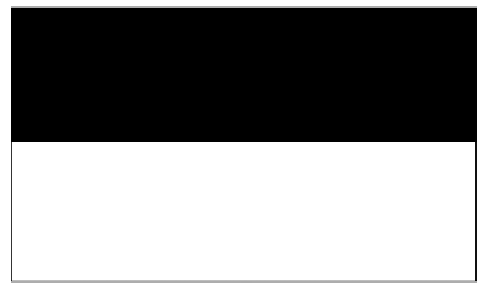
\includegraphics[scale=1]{alpr_mask.pdf}
			\caption{Ejemplo de máscara que puede ser seteada.}
			\label{fig:img_mask}
		\end{figure}
		
		\item \textbf{Prewarp} 
		
		Este parámetro permite adicionarle al software la configuración realizada sobre la cámara de video. De esta manera es posible reconocer más eficientemente las matriculas de los vehículos que no se encuentran de frente a la cámara. A pesar de que actualmente no se lo está utilizando, a futuro, este parámetro será modificado.
		
		\item \textbf{max\_plate\_width\_percent y max\_plate\_height\_percent}
		
		Por defecto, estos valores son 100. Se los seteó en 30 a ambos. De esta manera, se le informa al sistema que las posibles patentes no pueden ocupar más de un 30\% de la imagen. Por lo tanto, descartarán las posibles patentes que posean un valor superior al establecido.
		
		
	\end{itemize}
	
	\item \textbf{\underline{Archivos para el funcionamiento del ALPRD:}}
	
	Para poder ejecutar este modo de funcionamiento y reconocer las patentes argentinas, se debió modificar el archivo ``alprd.conf''. En el mismo, se le provee al sistema del URL que genera el streaming realizado por la cámara, en los parámetros ``country'' y ``pattern'' se establecen los archivos correspondientes creados para las patentes argentinas y, por último, se configura el parámetro ``topn'' en 1, ya que solo interesa obtener la mejor patente y no una lista de posibles matrículas. Además, se le configuró un ID a la cámara para poder distinguirla de las demás. 
	
	Por otro lado, como el estacionamiento considerado posee una vía de entrada y otra de salida, para que las cámaras situadas en las vías no suban sus trabajos a la misma cola de trabajo, se modificó el archivo ``daemon.cpp'' de manera que el sistema cree dos colas, una para la entrada y otra para la salida. Cabe destacar que una vez que se modifica este archivo se debe volver a compilar el software de manera que estos cambios tengan efecto sobre el funcionamiento del sistema. 
	
	Finalmente, para poder diferenciar entre las colas de entrada y salida, se debe crear un nuevo archivo ``alprd.conf'' con el ID de la cámara y el URL, referidos a las cámaras de salida. Para poder tener funcionando simultáneamente el sistema de entrada y el de salida, se debe tener una copia de los archivos ``alprd.conf'' y ``openalpr.conf'' (archivo que posee los mismos valores que openalpr.defaults.conf) para la entrada y, en una carpeta diferente, otra copia destinada a la salida, donde el ``alprd.conf'' debe estar seteado con los valores correspondientes a la salida. Por lo tanto, se deben ejecutar ambos archivos ``alprd'' en forma independiente, indicando la ubicación del archivo en el caso de que no se encuentre en la carpeta por defecto. De esta forma, las cámaras que se encuentran en la vía de entrada subirán sus trabajos a la cola de entrada y las de salida a su respectiva cola.
\end{enumerate}		
		
Una vez realizadas estas modificaciones, se volvió a evaluar el sistema utilizando los mismos sets de pruebas que al inicio, lo que permitió verificar las mejoras logradas. Los resultados se observan en la tabla \ref{tabla:openalpr_Tdesarrollado}. Cabe destacar que el parámetro detection\_iteration\_increase es el que produce el mayor impacto sobre el sistema, por lo que los nuevos resultados se presentan para tres diferentes valores de este parámetro.
		
\begin{table}[htb]
	\centering
	\resizebox{14cm}{!} {
		\begin{tabular}{|c|c|c|c|c|c|c|c|c|c|}
			\hline
			& \multicolumn{3}{c|}{1.1} & \multicolumn{3}{c|}{1.07} & \multicolumn{3}{c|}{1.04}\\
			\cline{2-10}
			& = & X & NF & = & X & NF & = & X & NF\\
			\hline \hline
			MERCOSUR & 80\% & 0\% & 20\% & 90\% & 0\% & 10\% & 90\% & 0\% & 10\%\\ \hline
			Antiguas & 70\% & 0\% & 30\% & 85\% & 0\% & 15\% & 95\% & 0\% & 5\%\\ \hline
		\end{tabular}
	}
	\caption{Variación de los resultados de los set de 20 imágenes.}
	\label{tabla:openalpr_Tdesarrollado}
\end{table}
	
Por último, se utilizaron los sets de 165 imágenes para obtener un resultado que sea más significativo. Dichos resultados se muestran el la tabla \ref{tabla:openalpr_Tdesarrollado160}.
	
\begin{table}[htb]
	\centering
	\resizebox{14cm}{!} {
		\begin{tabular}{|c|c|c|c|c|c|c|c|c|c|}
			\hline
			& \multicolumn{3}{c|}{1.1} & \multicolumn{3}{c|}{1.07} & \multicolumn{3}{c|}{1.04}\\
			\cline{2-10}
			& = & X & NF & = & X & NF & = & X & NF\\
			\hline \hline
			MERCOSUR & 92.73\% & 3.03\% & 4.24\% & 95.76\% & 0\% & 4.24\% & 95.76\% & 0\% & 4.24\%\\ \hline
			Antiguas & 88.48\% & 0.61\% & 10.91\% & 93.94\% & 0\% & 6.06\% & 94.55\% & 1.21\% & 4.24\%\\ \hline
		\end{tabular}
	}
	\caption{Resultados obtenidos para los sets de 165 imágenes.}
	\label{tabla:openalpr_Tdesarrollado160}
\end{table}	
	
Utilizando una muestra significativa de imágenes, se pudo verificar que al setear el parámetro mencionado anteriormente en 1.04 en lugar de 1.07 no se producen variaciones significativas en el reconocimiento. Mientras que en las patentes del MERCOSUR los resultados fueron los mismos que con el valor original del parámetro, en las antiguas solo hubo una mejoría de 0.61\%. Considerando que el tiempo de procesamiento es un factor muy importante y que el mismo debe ser el menor posible, se establece 1.07 como valor para el parámetro detection\_iteration\_increase.	
	
Cabe destacar que la experimentación fue realizada a partir de imágenes fijas. Sin embargo, el resultado de la misma es igualmente valido para el modo de funcionamiento a partir de un video en tiempo real debido a que procesar un frame del video es lo mismo que procesar una imagen fija.	
	
Luego de analizar el comportamiento del sistema con patentes de automóviles y camionetas se comprobó el funcionamiento del mismo con patentes de motocicletas. Este análisis se llevó a cabo sobre un número reducido de imágenes debido a que solo se buscó analizar su factibilidad, dejando a futuro el desarrollo de un conjunto de prueba mayor. Se construyeron dos sets de diez imágenes cada uno, uno con patentes del MERCOSUR y el otro con antiguas. Debe destacarse que se crearon los mismos archivos que en el caso de los otros vehículos, a excepción del archivo de configuración para las patentes del MERCOSUR. Esto se debió a que el sistema ya proveía el archivo correspondiente a las matriculas del MERCOSUR de las motos de Brasil, teniendo en cuenta que todas las matrículas del MERCOSUR son muy similares, como se mencionó anteriormente. Por último, debe mencionarse que las pruebas fueron realizadas con los parámetros de los demás archivos ya modificados, y no con los que se encontraban seteados por defecto. Los resultados obtenidos se pueden observar en la tabla \ref{tabla:pat_motos}.
	
\begin{table}[htbp]
	\begin{center}
		\begin{tabular}{|c|c|c|c|}
			\hline
			 & = & X & NF\\
			\hline 
			MERCOSUR & 100\% & 0\% & 0\%\\ 
			\hline 
			Antiguas & 90\% & 0\% & 10\%\\ \hline
		\end{tabular}
		\caption{Resultados obtenidos para el análisis de los sets con imágenes de motocicletas.}
		\label{tabla:pat_motos}
	\end{center}
\end{table}
	
	
\subsubsection{OpenCV 3 License Plate Recognition}	
	
Al igual que para el otro sistema, se realizaron las pruebas iniciales con la configuración por defecto sobre los mismos sets de 20 imágenes. En este caso, los resultados obtenidos son los observados en la tabla \ref{tabla:opencv_Torig}.	
	
\begin{table}[htb]
	\begin{center}
		\begin{tabular}{|c|c|c|c|}
			\hline
			& \multicolumn{3}{c|}{Set de 20 imágenes}\\	
			\cline{2-4}
			& = & X & NF \\
			\hline 
			MERCOSUR & 25\% & 70\% & 5\% \\ 
			\cline{1-4}
			Antiguas & 0\% & 45\% & 55\% \\ 
			\cline{1-4}
		\end{tabular}
	\caption{Resultados del reconocimiento desarrollado con la configuración por defecto.}
	\label{tabla:opencv_Torig}
	\end{center}
\end{table}		
	
Este software fue diseñado para el reconocimiento de matrículas estadounidenses, por lo que fue necesario modificarle las dimensiones de los caracteres para adaptarlos a los de las patentes argentinas. 

Por otra parte, como se mencionó previamente, para el reconocimiento de caracteres se recurre al algoritmo K-NN, el cual utiliza dos archivos: ``classification.xml'' e ``images.xml''. Los mismos son usados para entregar una respuesta para los caracteres que son analizados por el sistema. Por lo tanto, si se observan estos archivos, se puede verificar que fueron realizados para un formato de letra que no es el propio de las patentes argentina. Esto puede producir errores en el reconocimiento. En consecuencia, se desarrollaron dos nuevos archivos de cada tipo. El primer par se generó mediante una imagen que contenía todas las letras en mayúscula y todos los números con la fuente de las patentes del MERCOSUR (FEEngschrift). El segundo par se generó de la misma forma, pero con la fuente del modelo antiguo de patentes argentinas (LicensePlate).
	
Para crear dichos archivos, se utilizó el código ``OpenCV 3 KNN Character Recognition'',  basado en la librería OpenCV, desarrollado por Chris Damhs \cite{opencv3KNN}. 	Mediante el archivo ``GenData.cpp'' se pueden generar fácilmente los archivos mencionados para luego utilizarlos en el código descripto anteriormente.

Finalmente, se estableció la cantidad mínima y máxima de caracteres que debe poseer la matrícula.
	
Luego de aplicar estas modificaciones, los resultados que se obtuvieron para los mismos sets de 20 imágenes y para los nuevos de 165 son los que se muestran en la tabla \ref{tabla:opencv_Tdesarrollado}.

\begin{table}[htb]
	\centering
	\resizebox{14cm}{!} {
		\begin{tabular}{|c|c|c|c|c|c|c|}
			\hline
			& \multicolumn{3}{c|}{Set de 20 imágenes} & \multicolumn{3}{c|}{Set de 165 imágenes}\\
			\cline{2-7}
			& = & X & NF & = & X & NF\\
			\hline \hline
			MERCOSUR & 60\% & 35\% & 5\% & 37.58\% & 55.55\% & 7.87\%\\ \cline{1-7}
			Antiguas & 0\% & 45\% & 55\% & 0\% & 68.48\% & 31.52\%\\ \cline{1-7}
		\end{tabular}
	}
	\caption{Resultados de la detección con el entrenamiento desarrollado.}
	\label{tabla:opencv_Tdesarrollado}
\end{table}	
	
Cabe destacar que no se efectuó la experimentación con patentes de motocicletas con este software debido a que no posee la capacidad de entregar resultados de patentes multilinea.	
	
\subsection{Comparación de los modelos}		
	
Si bien ambos sistemas son capaces de reconocer la patente que se observa en la imagen analizada, con el software OpenALPR se logra obtener un porcentaje de éxito mayor. Esto se puede confirmar al ver los resultados obtenidos por ambos sistemas para los sets de 165 imágenes. Por un lado, en el caso de las matriculas del MERCOSUR, con el OpenALPR se obtiene una mejora del 60\% aproximadamente en el reconocimiento correcto respecto del OpenCV. Por otro lado, en el caso del modelo antiguo, se obtuvo una mejora del 95\%.

Luego de analizar el comportamiento de los sistemas, se determinó que la única ventaja que posee el código basado en OpenCV es que, al determinar primero la ubicación de los caracteres y luego la patente, este es capaz de detectar todo tipo de patentes independientemente de su tamaño. En este aspecto el software OpenALPR requiere un conjunto de archivos específicos para cada formato de matricula.

Por otra parte, OpenALPR presenta varias ventajas sobre el otro sistema que son, junto con la efectividad, las razones por las que se decidió trabajar con este software. Entre estas ventajas podemos destacar:	
	
\begin{itemize}
	\item Es más veloz
	\item Al detectar la ubicación de la patente y sus bordes, puede descartar con mayor facilidad posibles patentes
	\item Otorga una lista de posibilidades sobre la patente con un porcentaje de confianza, lo que permite detectar errores del OCR
	\item Posee la opción de invertir los colores de las patentes de manera de analizar cualquier formato bajo los mismos colores. De esta manera se evita tener que hacer un procesamiento previo de la imagen
	\item Brinda la posibilidad de validar las combinaciones de caracteres obtenidas según el formato que tengan
	\item Permite leer patentes multilínea, como es el caso de las matrículas de las motocicletas
	\item Permite el tratamiento de video y video en tiempo real, que fue la opción elegida para este proyecto
\end{itemize}	

En lo que respecta a los errores, en el caso del código de OpenCV, se debe mencionar que el sistema es muy sensible al entorno de la imagen. Cualquier cartel o conjunto de letras concatenadas que supere la longitud de caracteres de la patente va a ser considerado como la patente, ya que el sistema analiza una única posible matricula y es la que contenga la mayor cantidad de caracteres. También es posible que dentro del entorno se consideren como posibles caracteres partes del fondo de la imagen, debido a que el sistema trabaja con contornos y sus dimensiones para detectar los caracteres. Además, al no utilizar un motor de OCR propio, se producen confusiones entre los caracteres que son similares entre sí, como en el caso del ``0'', ``O'' y ``Q'' o bien ``B'' y ``8'', entre otros.	
	
Por otra parte, deben considerarse los posibles errores que se producen al trabajar con OpenALPR. En cuanto a las matrículas del MERCOSUR, se pudo identificar que los caracteres poseen escritos a lo ancho de ellos las palabras ``MERCOSUR'' y “Argentina” en color gris. Esto puede presentar grandes inconvenientes debido a que, si se logran apreciar en la imagen, al momento de reconocer los caracteres el sistema falla y no logra entregar una respuesta. Un ejemplo de este caso se presenta en las figuras \ref{fig:img_palabras_int} y ~\ref{fig:img_postsegment}.

\begin{figure}[H]
	\centering
	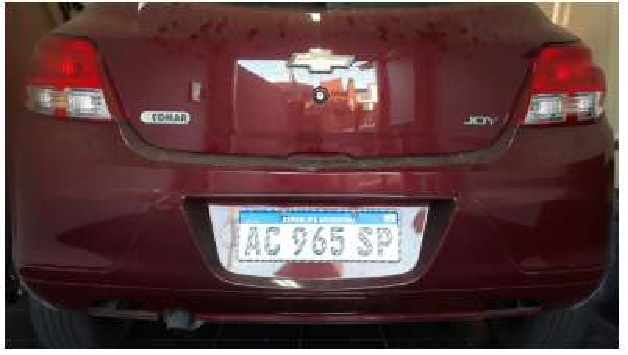
\includegraphics[scale=1]{palabras_internas.pdf}
	\caption{Patente con palabras internas apreciables.}
	\label{fig:img_palabras_int}
\end{figure}
\begin{figure}[H]
	\centering
	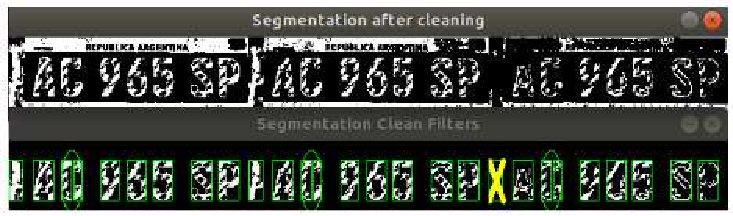
\includegraphics[scale=1]{postsegment.pdf}
	\caption{Reconocimiento de caracteres en patente con palabras internas apreciables.}
	\label{fig:img_postsegment}
\end{figure}

Como se puede observar en la figura \ref{fig:img_palabras_int}, la patente de la imagen resulta muy brillante por la forma en que la luz impacta sobre ella. Debe destacarse, en base las pruebas realizadas, que otro factor que puede influir para que esto suceda o no es el ángulo con el que se toma la imagen. Realizando variaciones sobre el mismo, se observó que el problema puede aparecer incluso si la patente no es tan brillante como se observa en el ejemplo anterior.

La solución a este problema es tomar la fotografía a una distancia entre 2.5 y 3 metros aproximadamente, dependiendo de qué tan iluminada esté la patente y el ángulo que posea la cámara. A estas distancias, si bien se siguen apreciando las palabras dentro de los caracteres, al segmentarlos e intentar reconocerlos no aparecen tan manchados como en el caso de la figura~\ref{fig:img_postsegment}, donde la imagen fue tomada a 1 metro de distancia.

Un problema que se produjo con ambos tipos de patente es la visualización de una sombra sobre la misma. Esto genera que a la hora de segmentar los caracteres aparezcan cortados y no se obtengan resultados. Cabe destacar que, trabajando a una distancia como la ya mencionada, el sistema igualmente puede fallar pero se vuelve mucho más robusto ante circunstancias como estas.

Por último, en cuanto al modelo antiguo, surgió una mayor cantidad de problemas en relación al ángulo de la cámara. Esto hace referencia a que rotaciones pequeñas pueden generar conflictos al reconocer caracteres como la ``O''y la ``Q'', debido a que en estas matrículas los mismos son muy similares. Si bien este problema también se da en las patentes del MERCOSUR con letras como la ``V'', la cual se confunde con la ``W'', y la ``M'' que se confunde con la ``H'', el mismo tiene una ocurrencia mucho menor que con el otro modelo.


\section{Conclusiones}
	
A lo largo de este capítulo se han introducido los sistemas ALPR, pasando por sus diferentes aplicaciones y empresas que los desarrollan y/o utilizan a nivel mundial. Además, se ha explicado el funcionamiento de un sistema ALPR en forma general y se ha hecho hincapié en el funcionamiento y la experimentación de dos software con los que se trabajó. A partir de estos últimos, se pude observar que no todos los sistemas ofrecen los mismos servicios y calidad, ya que presentan variaciones a la hora de llevar a cabo las etapas generales, dependiendo de la visión adoptada por la empresa o persona que los haya desarrollado. Por estos motivos, a la hora de elegir un sistema es de vital importancia analizar la aplicación en la que se lo va a utilizar, de manera de determinar el tipo de software que se requiere (pago, gratuito o de código abierto). Además, debe considerarse la forma en la que los mismos funcionan, de manera de determinar cuál de estos se adapta mejor a las necesidades. 

Se puede observar que la adaptación de un sistema ALPR para modelos de patentes que no vienen incorporadas en el sistema no es una tarea trivial, ya que se requiere la modificación y ajuste de una gran cantidad de parámetros. Además, se debe tener en cuenta la posibilidad de que el mismo no incluya los archivos de entrenamiento para el motor de OCR y el detector para el nuevo tipo de patentes. En este caso, sería necesario desarrollar dichos entrenamientos, lo cual es una tarea muy compleja. En el caso particular de este proyecto, debido a la similitud de las patentes argentinas con otros tipos de patentes, se pudieron reutilizar esos archivos entrenamientos a partir de los destinados a otros países. Sin embargo, en un futuro se debería realizar un entrenamiento propio para lograr mejores resultados para todos los modelos de patentes argentinas.





















